\chapter{Conditioning generation with multiple task-specific constraints}
\label{chap:chapter3}


\begin{chapterabstract}
	The problem addressed in this chapter is the generation of polarimetric images using Cyle-Consistent Generative Adversarial Networks (CycleGAN) with constraints derived from the optics of polarimetry. The conducted research is motivated by the increasing popularity of the combination of deep learning frameworks with polarimetric imaging in various domains, including medical imaging and scene analysis. Even if polarimetric imaging has shown improved performances, their robustness may be questioned because of the small size of the training datasets. 
	This issue could be resolved by data augmentation. However, polarization modality is subject to some physical feasibility constraints that could be impeded with classical data augmentation techniques. In this paper we propose a framework based on CycleGAN, integrating the constraints of polarimetric images during training stage. We evaluate the proposed generative model on road scene images. 
	The obtained results achieved an effective generation of physical polarization-encoded images. Further experiments on the task of road object detection show that with the generated images, the detection of cars and pedestrian are improved by up to 9\%.
\end{chapterabstract}

%===========================================================
\section{Introduction}


Generative  adversarial networks (GAN) \citep{Goodfellow2014,Wang2019} are powerful deep generative models used to  implicitly learn complex data distributions and to generate realistic samples from them. In its standard form, a GAN consists of two models: a generator which maps samples drawn from a latent low-dimensional distribution (usually uniform or gaussian distributions) to  high-dimensional points expected to follow the sought data distribution, and a discrimination model which discriminate the real samples from the generated ones \citep{Goodfellow2014}.  GANs have proven remarkable in various application domains including  image generation \citep{Arjovsky17}, image-to-image translation \citep{Isola2016, Zhu2017, Hoffman18} or image attribute manipulation \citep{Antipov2017} to name a few. 

Arguably most of the impressive achievements of the GAN were obtained for RGB images. A body of work attempted to extend GAN architectures to other uncommon imaging domains. For instance, some existing methods rely on CycleGAN \citep{Zhu2017a}, an image-to-image translation network, to generate infrared road scenes from RGB counterpart images \citep{Zhang2018b}, to produce thermal images for person re-identification \cite{Knia2018} or for infrared image colorization \cite{Mehri2019}. In the same vein,  \citet{Nie2017} achieved data augmentation in the field of medical imaging by transforming MRI inputs into pseudo-CT images.  From another point of view, \citet{Sallab2019} used CycleGANs to produce realistic LiDAR points cloud from simulated ones. 


Following the previous stream of work, this paper contributes generative models for non-conventional imaging techniques. Specifically we propose a  generative model framework to produce realistic polarimetric images.  The significant interest resides in the fact that polarimetric imaging is a rich modality that enables to characterize an object by its reflective properties. Those properties are object specific, hence, they convey strong features to analyse the content of a scene. In a polarimetric image, each pixel encodes information regarding the object's roughness, its orientation and its reflection \citep{wolff1995polarization}. Applications of polarimetric imaging range from indoor autonomous navigation \citep{berger2017depth}, depth map estimation \citep{Zhu_2019_CVPR}, 3D objects reconstruction \citep{morel2006active} to differentiation of healthy and unhealthy cervical tissues in order to detect cancer at an early stage \citep{rehbinder2016ex}. Also, recently, polarization imaging was exploited in autonomous driving applications either to enhance car detection \citep{fan2018polarization}, road mapping and perception \citep{aycock2017polarization} or to detect road objects in adverse weather conditions \citep{blin2019road}.  However, these  applications are characterized by the reduced size of the available training databases which restrains them from using deep neural networks, thus the need of polarimetric data generation model. 

Contrary to RGB, LiDAR or infrared image generation which mostly responded to visual qualitative  constraints, unless some learnable knowledge constraints are enforced (see \cite{hu2018deep} for pose conditional person image generation), sampling polarization images is more challenging. Indeed, this imaging technique comes with physical admissibility constraints on the pixels of an image. To be physically feasible, each pixel entry of such an image should satisfy some physical constraints related to light polarization principle and to the calibration setup of the acquisition devices.
Therefore, we formulate our problem of polarimetric image generation as a CycleGAN learning problem under physical constraints to ensure that the generated images are valid. CycleGANs \citep{zhu2017unpaired} enabled to achieve unpaired image-to-image translation with only a few number of images. 
They allow to circumvent the expensive labelling step by transferring a source labelled dataset to one or multiple target domain \citep{almahairi2018augmented} by keeping unchanged the shapes of the source image. 


Starting from unpaired sets of RGB and polarimetric images, we propose a learning framework based on CycleGAN and able to handle the physical polarization constraints during training. We demonstrate the effectiveness of our constrained-output CycleGAN on the KITTI dataset \citep{geiger2012we} and the Berkeley Deep Drive dataset (BDD100K) \cite{xu2017end}, two common datasets used for object detection in road scenes. Using the generated polarization-encoded images to train a deep object detectors, we witness an improvement of the detection performances of cars and pedestrians which are of great interest for autonomous driving applications. 

To summarize, the contributions of this paper are:
\begin{itemize}
	\item as far as our knowledge can go, we propose the first framework for generating physical polarization-encoded images starting from RGB images, 
	\item we propose an extension of CycleGAN which allows to generate polarimetric-encoded images while handling the physical constraints the pixels of the generated image should satisfy,
	\item when plugged into the training procedure of an object detector for pre-training, the generated images help improving the detection performances.
\end{itemize}

The remainder of the paper is organized as follows:  
the polarization formalism and the physical constraints it involves are first presented. Then, the image-to-image translation using Cycle-Consistent GAN is described and a way to take into account these physical constraints during the training process of the CycleGAN for generating polarimetric images is investigated. Experimental evaluations are conducted ; they aim to translate RGB images of KITTI and BDD100K datasets into polarimetric images. Finally, the generated images are exploited to boost the performances of an object detection network. The code for the experiments is available at: \url{https://anonymous.4open.science/r/4a83820e-9c65-417c-af3a-ab2979d6e2e8/}

%%%%%%%%%%%%%%%%%%%%%%%%%%%%%%%%%%%%%%%%%%%%%%%%%%%%%%%%%%%%%%%%%%%%%%%%%%%%%%%%%%%%%%%%%%%%%%%%%%%

\section{Framework}

This section introduces the polarization formalism, the Generative Adversarial Network approach and the CycleGAN principles. It focuses on the formulation of the proposed modelling framework, namely the learning of a CycleGAN with output constraints. A solution approach is detailed and the related learning principle is presented. 

\subsection{Polarization formalism}
\label{physical_prop}

Light waves can oscillate in different orientations. Polarization represents the direction of propagation of the electrical field of the light wave. When the direction is linear, elliptical or circular, the polarization state is said to be totally polarized. However, it is partially polarized or non polarized when the light wave partly propagates in a random way \citep{bass1995handbook}. 

Polarimetric imaging consists in representing the polarization state of the light wave reflected from each part of the scene. When an unpolarized light wave is being reflected, it becomes partially linearly polarized. Its polarization depends on the normal surface  and the refractive index of the material it impinges on. The linear part of the reflected light can be described by measurable parameters and specifically by the linear Stokes vector $S = \begin{bmatrix}
S_0 & S_1 & S_2 \end{bmatrix}^\top$ where $S_0>0$ represents the total intensity, $S_1$ the amount of horizontally and vertically linearly polarized light and $S_2$ the amount of linearly polarized light at $\pm$~45\degree. 
%
It is important to note that by design, the Stokes vector is physically admissible if and only if the two following conditions are met:  
%
\begin{equation}
S_0 > 0
\quad \mbox{ and } \quad 
S_0^2 \geqslant S_1^2 + S_2^2 \enspace.
\label{eqn:stokes_constraint_S0}
\end{equation}

One salient physical property, obtained from the Stokes parameters, is the degree of polarization (DOP) \citep{ainouz2013adaptive}  defined by:
$$
DOP = \frac{\sqrt{S_1^2+S_2^2}}{S_0} \enspace.
$$
%
The $DOP \in [0,1]$ refers to the amount of polarized light in a wave. It is equal to 1 for a totally polarized light, 0 for unpolarized light and between 0 and 1 for partially polarized light.

Polarization images are accordingly obtained by the computation of the Stokes vector related to each pixel. The acquisition principle is based on a device composed of a polarizer oriented at an angle $\alpha$ between the object and the sensor \citep{Wang_2019_CVPR}. At least three acquisitions with three different angles are required to get the Stokes parameters. The reflected light from the object, represented by the unknown Stokes vector, passes through the rotated polarizer before reaching the camera. 

For this work, a Polarcam 4D Technology polarimetric camera was used, enabling to get simultaneously four images respectively obtained with four different linear polarizers oriented at $(\alpha_i)_{i=1:4} =$ (0\degree, 45\degree, 90\degree, 135\degree). The polarimetric camera measures an intensity $I_{\alpha_i}$ of the scene for each angle $\alpha_i$. The relationship between the Stokes vector $S$ and the intensities $I(\alpha_i)_{i=1:4}$ reaching the camera is given by: 
$$
I_{\alpha_i} = \tfrac{1}{2}\begin{bmatrix}
1 & \cos(2\alpha_i) & \sin(2\alpha_i)
\end{bmatrix} \begin{bmatrix}S_0 \\ S_1 \\ S_2\end{bmatrix} \enspace,
\forall i=1, 4 \nonumber 
$$
\noindent that is:
\begin{equation}
I = AS \enspace, 
\label{eqn:IAS}
\end{equation}
\noindent where $I = \begin{bmatrix} I_0 & I_{45} & I_{90} & I_{135}\end{bmatrix}^\top$ refers to the four intensities according to each angle of the polarizer $(\alpha_i)_{i=1:4}$ and $A \in \mathbb{R}^{4\times 3}$, to the calibration matrix of the polarization camera, defined as: 
$$
A = \frac{1}{2} {\begin{bmatrix}
	1 & \cos(2\alpha_1) & \sin(2\alpha_1) \\
	1 & \cos(2\alpha_2) & \sin(2\alpha_2) \\
	1 & \cos(2\alpha_3) & \sin(2\alpha_3) \\
	1 & \cos(2\alpha_4) & \sin(2\alpha_4)
	\end{bmatrix}}
\\
=  \frac{1}{2} {\begin{bmatrix}
	1 & 1 & 0 \\
	1 & 0 & 1 \\
	1 & -1 & 0 \\
	1 & 0 & -1
	\end{bmatrix}} \enspace. \nonumber
$$
%
An example of the different intensities for the same scene is shown in Figure~ \ref{fig:polar_overview intensities}. 

\begin{figure}
	\centering
	\begin{subfigure}{0.25\textwidth}
		\centering
		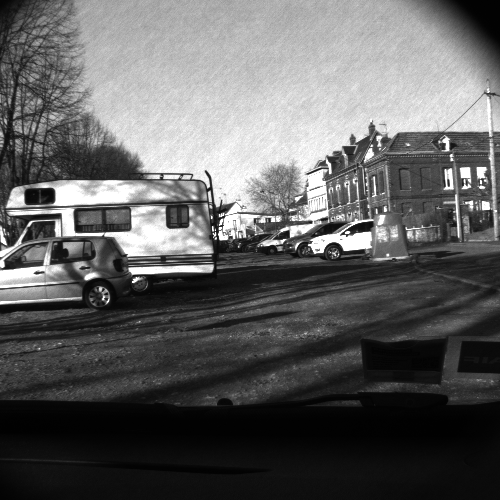
\includegraphics[width=\linewidth]{images/2474_I0.png}
	\end{subfigure}%
	\begin{subfigure}{0.25\textwidth}
		\centering
		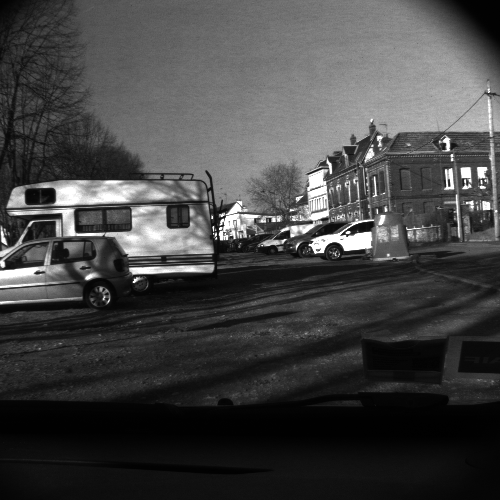
\includegraphics[width=\linewidth]{images/2474_I45.png}
	\end{subfigure}%
	\begin{subfigure}{0.25\textwidth}
		\centering
		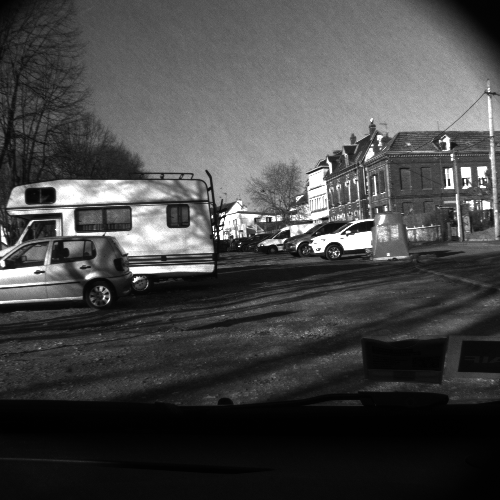
\includegraphics[width=\linewidth]{images/2474_I90.png}
	\end{subfigure}%
	\begin{subfigure}{0.25\textwidth}
		\centering
		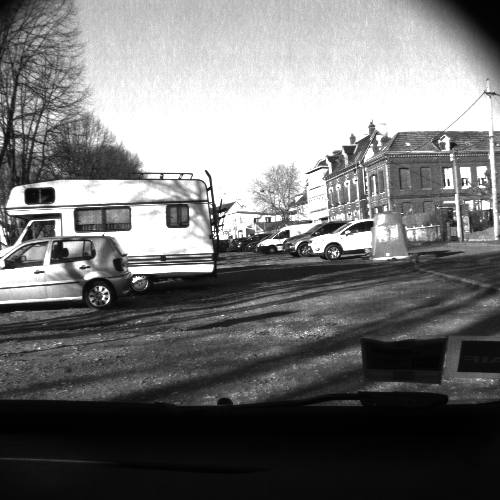
\includegraphics[width=\linewidth]{images/2474_I135.png}
	\end{subfigure}
	\caption{Example of a polarimetric image. From left to right, the intensities corresponding to the polarizer rotation angles 0$\degree$, 45$\degree$, 90$\degree$ and 135$\degree$.}
	\label{fig:polar_overview intensities}
\end{figure}
%
To get the unknown Stokes parameters from the measured intensities (equation \ref{eqn:IAS}), we require $\tilde{A} = (A^\top A)^{-1} A^\top \in \mathbb{R}^{3\times 4}$ the pseudoinverse of the matrix $A$. The relationship between $S$ and $I$ is then defined by:
\begin{eqnarray}
S & = & \tilde{A}I = 
\begin{bmatrix}
1 & 0 & 1 & 0 \\
1 & 0 & -1 & 0 \\
0 & 1 & 0 & -1
\end{bmatrix}
\begin{bmatrix} 
I_0 \\
I_{45} \\
I_{90} \\
I_{135}
\end{bmatrix} 
= 
\begin{bmatrix} 
I_0 + I_{90} \\
I_0 - I_{90} \\
I_{45} - I_{135} 
\end{bmatrix}
\label{eqn:stokes2} \enspace.
\end{eqnarray}
%
Combining equations (\ref{eqn:IAS}) and (\ref{eqn:stokes2}), we attain the following condition  
$$
I = A\tilde{A}I \enspace,
$$
\noindent which is satisfied if and only if:
\begin{equation}
I_0 + I_{90} = I_{45} + I_{135} \enspace.
\label{eqn:physics}
\end{equation}
%
Stokes images should then satisfy two main conditions: the physical admissibility constraints in equation \eqref{eqn:stokes_constraint_S0}
and the calibration constraint given by equation \eqref{eqn:physics}. The generation of new polarimetric images have to comply with these essential constraints. 

%%%%%%%%%%%%%%%%%%%%%%%%%%%%%%%%%%%
%%%%%%%%%%%%%%%%%%%%%%%%%%%%%%%%%%%%%%%%%%%%%%%%%%%%

\subsection{Unpaired image-to-image translation with CycleGAN}

Given two domains $X$ and $Y$, unpaired image-to-image translation is the task of learning the mapping functions $M_{XY} : X \rightarrow Y$ and $M_{YX} : Y \rightarrow X$ using unpaired samples $x_i \in X$ with $i \in [1..N]$ and $y_j \in Y$ with $j \in [1..M]$. 
%
An effective approach to achieve the task is CycleGAN \citep{zhu2017unpaired}. 
It consists in learning the two mapping models $M_{XY}$ and $M_{YX}$ by combining the objective function of the standard Generative Adversarial Network (GAN) \citep{goodfellow2014generative}  with a Cycle-Consistency loss function. The adversarial cost related to the GAN serves for training the models to generate samples that will match the target domain distribution, while the Cycle-Consistency cost ensures that the learned models are able to correctly reconstruct an original image (of the source domain) from a generated one.

Formally a GAN is composed of a generative model $G : Z \rightarrow X$ which maps a known distribution $p_Z$, usually normal or uniform, to the unknown distribution $p_X$ of the samples and a discrimination model $D : X \rightarrow [0,1]$. The generator $G$ attempts to fool the discriminator $D$, which in turn tries to distinguish a real sample from a sample generated by the model $G$. Learning a GAN amounts to solve the following problem:
$$
\begin{array}{c}
G^*, D^* = \arg\min_G\max_D L_{GAN}(D, G) \enspace,  \nonumber \\
\text{with }L_{GAN}(D, G) = \mathop{\mathbb{E}}_{x \sim p_X} \Big[\log (D(x))\Big] +
\mathop{\mathbb{E}}_{z\sim p_Z} \Big[\log (1-D(G(z)))\Big] \enspace, \nonumber
\end{array}
$$
\noindent where $\mathbb{E}$ refers to the expectation.

For its part, CycleGAN learns the two models $M_{XY}$ and $M_{YX}$ by using unpaired real samples $x$ $\in X$ and $y \in Y$ respectively drawn according to the (unknown) distributions $p_X$ and $p_Y$  as input. It also learns two discrimination networks $D_X: X \rightarrow [0,1]$ and $D_Y: Y\rightarrow [0,1]$ able to detect generated samples from real ones in the domains $X$ and $Y$ respectively. CycleGAN relies on the Least-Squares variant of GAN \citep{mao2017least} and considers the following adversarial  costs:
%
\begin{eqnarray}
L_{GAN}(D_Y, M_{XY}) = \mathop{\mathbb{E}}_{y \small{\sim} p_Y} \Big[(D_Y(y) - 1)^2\Big] + \mathop{\mathbb{E}}_{x\small{\sim}p_X}\Big[D_Y(M_{XY}(x))^2\Big] \enspace, \nonumber\\
L_{GAN}(D_X, M_{YX}) = \mathop{\mathbb{E}}_{x \small{\sim}p_X} \Big[(D_X(x) - 1)^2\Big] + \mathop{\mathbb{E}}_{y\small{\sim}p_Y} \Big[D_X(M_{YX}(y))^2\Big] \enspace. \nonumber
\end{eqnarray}
%
In order to ensure the cyclic consistency that is both the compositions $M_{XY} \circ M_{YX}$ and $M_{YX} \circ M_{XY}$ are identity functions, a $\ell_1$ reconstruction error term is devised for the mapping models: 
\begin{equation}
L_{reco}(M_{XY}, M_{YX})\small{=}\mathop{\mathbb{E}}_{y \small{\sim} p_Y}||y - M_{XY}(M_{YX}(y))||_1 +\mathop{\mathbb{E}}_{x \small{\sim} p_X}||x - M_{YX}(M_{XY}(x))||_1
\enspace. \nonumber
\end{equation}
%
Gathering all these elements leads to the objective function 
\begin{align}
L_{CycleGAN}&(D_X, D_Y, M_{XY}, M_{YX}) = \nonumber \\ 
&L_{GAN}(D_Y, M_{XY}) + L_{GAN}(D_X, M_{YX})+\lambda L_{reco}(M_{XY}, M_{YX})
\enspace, \label{eqn:Lcyclegan}
\end{align}


\noindent where $\lambda > 0$ is an hyper-parameter that controls the influence of the reconstruction term. Training a CycleGAN consists in solving, via alternate gradient descent,  the following minmax problem 

\begin{eqnarray}
M_{XY}^*, M_{YX}^*, D_X^*, D_Y^* =\arg\min_{\substack{M_{XY}\\M_{YX}}}\max_{\substack{D_X\\D_Y}} L_{CycleGAN}(D_X, D_Y, M_{XY}, M_{YX}) \enspace. \label{eq:cycleGAN}
\end{eqnarray}

The full learning procedure of a CycleGAN  is sketched in Algorithm \ref{alg:cyclegan_train}.

\begin{algorithm}[]
	\begin{algorithmic}[H]
		\REQUIRE{$X$ and $Y$ two unpaired datasets, $M_{XY}$ and $M_{YX}$ the mapping networks, $D_X$ and $D_Y$ the discrimination models, $m$ the mini-batch size}
		\REPEAT
		\STATE sample a mini-batch $\lbrace x_i \rbrace_{i=1}^m$ from $X$\;
		\STATE sample a mini-batch $\lbrace y_i \rbrace_{i=1}^m$ from $Y$\;
		\STATE update $D_X$ by stochastic gradient descent of
		\STATE \ \ \ \ $ \sum_{i=1}^{m}(D_X(x_i)-1)^2 + (D_X(M_{YX}(y_i)))^2$
		\STATE update $D_Y$ by stochastic gradient descent of
		\STATE \ \ \ \ $ \sum_{i=1}^{m}(D_Y(y_i)-1)^2 + (D_Y(M_{XY}(x_i)))^2$
		\STATE sample a mini-batch $\lbrace x_i \rbrace_{i=1}^m$ from $X$\;
		\STATE sample a mini-batch $\lbrace y_i \rbrace_{i=1}^m$ from $Y$\;
		\STATE update $M_{XY}$ by stochastic gradient descent of
		\STATE \ \ \ \ $ \sum_{i=1}^n (D_Y(M_{XY}(x_i))-1)^2 + \lambda (||x_i - M_{YX}(M_{XY}(x_i))||_1$ \STATE \ \ \ \ \ \ \ \ $+||y_i -M_{XY}(M_{YX}(y_i))||_1)$\;
		\STATE update $M_{YX}$ by stochastic gradient descent of
		\STATE \ \ \ \ $ \sum_{i=1}^n (D_X(M_{YX}(y_i))-1)^2+ \lambda (||x_i - M_{YX}(M_{XY}(x_i))||_1 $
		\STATE \ \ \ \ \ \ \ \ $+ ||y_i - M_{XY}(M_{YX}(y_i))||_1)$\;
		\UNTIL a stopping condition is met
	\end{algorithmic}
	\caption{CycleGAN training algorithm}
	\label{alg:cyclegan_train}
\end{algorithm}

\subsection{Proposed approach}
\label{polarGAN}

As discussed above, our main goal is to learn a generative model able to produce realistic polarization-based images starting from RGB images. For the sake, we adopt the image-to-image translation framework and extend it to account for the constraints a polarimetric image must fulfill. 

To generate a polarimetric image  from an RGB image, we propose to use the CycleGAN approach to learn the translation models $M_{XY}$ and $M_{YX}$ between $X$ the domain of the polarimetric images and $Y$ the RGB image domain. Let $\hat{I} \in \mathbb{R}^4$ be the intensity vector associated to a pixel of a generated polarimetric image. To be physically admissible, each pixel  has to satisfy the admissibility constraints (\ref{eqn:stokes_constraint_S0}) and the calibration constraint (\ref{eqn:physics}). 
%
We refer in the sequel these polarimetric constraints by $\mathcal{C}_1$, $\mathcal{C}_2$ and $\mathcal{C}_3$ as follows:
\begin{eqnarray}
\mathcal{C}_1 &:& I = AS\enspace, \nonumber\\
\mathcal{C}_2 &:& S_0^2 \geqslant S_1^2 + S_2^2 \enspace, \nonumber\\
\mathcal{C}_3 &:& S_0 > 0 \enspace. \nonumber
\end{eqnarray}

By design, the first component of the Stokes vector is always positive as it represents the total intensity reflected from an object.  As the last layer of the generation models customary uses the tangent hyperbolic as activation function, each output intensity $\hat I$ is within the range $]-1,1[$ which we scale to $]0,255[$. Hence $\hat{S}_0=\hat{I}_0+\hat{I}_{90}$ (see equation (\ref{eqn:stokes2})) is ensured to be strictly positive. Therefore, constraint $\mathcal{C}_3$ can be deemed satisfied for the real and the generated polarimetric images. To handle the remaining constraints $\mathcal{C}_1$ and $\mathcal{C}_2$, one could resort to the Lagrangian dual of CycleGAN optimization problem (\ref{eq:cycleGAN}) subject to these constraints. However, this may be computationally expensive, as it requires to entirely optimize four neural networks (respectively the discrimination and the mapping network models) in an inner loop of a dual ascent algorithm. Moreover the overall optimization procedure may not be stable because of the minmax game involved in the CycleGAN learning. 

In order to derive  an efficient algorithm to learn CycleGAN under output constraints, we introduce a relaxation of the problem. Instead of strictly enforcing the constraints, we measure how far the generated image pixels are from the feasibility domain through additional cost functions we attempt to minimize.
%
For the constraint $\mathcal{C}_1$, a $\ell_2$ distance between the generated image $M_{YX}$ and $A\hat{S}$ is proposed. It reads
%
\begin{equation}
L_{\mathcal{C}_1} = \mathop{\mathbb{E}}_{y\sim p_Y} ||M_{YX}(y) - A\hat{S}||_2\enspace,  \nonumber
\label{eqn:ls}
\end{equation}
%
with $\hat{S}=\begin{bmatrix}
\hat{S_0} & \hat{S_1} & \hat{S_2}
\end{bmatrix}^\top$ the Stokes vector calculated from the generated image by $M_{YX}$ using equation \eqref{eqn:stokes2}.
%
Similarly, to enforce the constraint $\mathcal{C}_2$, a rectified linear penalty $L_{\mathcal{C}_2}$ is considered. It is defined by:
\begin{equation}
L_{\mathcal{C}_2} = \mathop{\mathbb{E}}_{y\sim p_Y}  \max\left(\hat{S_1}^2 + \hat{S_2}^2 -
\hat{S_0}^2, 0 \right)\enspace.\nonumber
\label{eqn:lreg}
\end{equation}
%
The loss $L_{\mathcal{C}_1}$ translates the respect of the acquisition conditions according to the calibration matrix $A$ while  $L_{\mathcal{C}_2}$ is related to the physical admissibility constraint on the deduced Stokes vectors from the generated image.

Gathering all these elements, we train our CycleGAN under physical constraints, by optimizing the following objective function:
\begin{equation}
L_{final}= L_{CycleGAN}+\mu L_{\mathcal{C}_1} + \nu L_{\mathcal{C}_2} \enspace.
\label{eqn:lfinal}
\end{equation}
%
The non-negative hyper-parameters $\mu$ and $\nu \in \mathbb{R}^{+}$ control respectively the balance of admissibility and calibration constraints according to the CycleGAN loss $L_{CycleGAN}$ (see equation~\eqref{eqn:Lcyclegan}). As the values of $L_{\mathcal{C}_1}$ and $L_{\mathcal{C}_2}$ are computed pixel-wisely, we consider their averages over the whole image in the objective function. The training principle of the proposed generative model is illustrated in Figure~\ref{fig:overview_polarCycle}.

\begin{figure} 
	\centering
	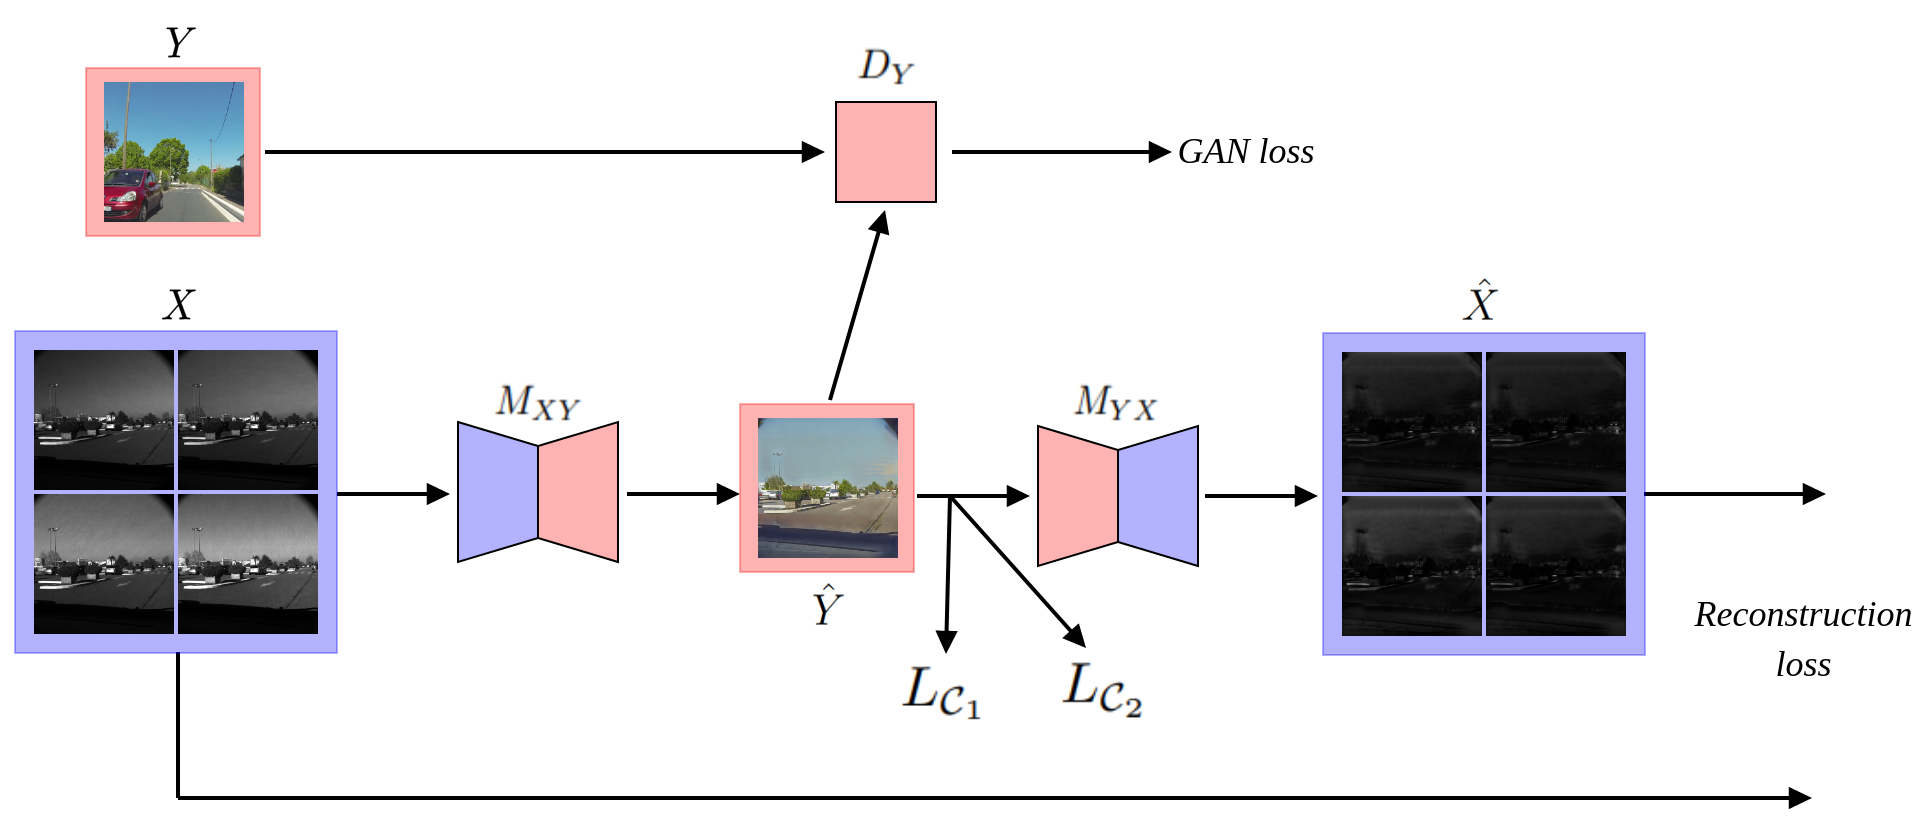
\includegraphics[scale=0.15]{images/PolarCycle.png}
	\caption{Overview of the CycleGAN training process extended with $L_{\mathcal{C}_1}$ and $L_{\mathcal{C}_2}$.}
	\label{fig:overview_polarCycle}
\end{figure}

%%%%%%%%%%%%%%%%%%%%%%%%%%%%%%%%%%%%%%%%%%%%%%%%%%%%%%%%%%%%%%%%%%%%%%%%%%%%%%%%%%%%%%%%%%%%%%%%%%%%%%%%%%%%%%%%%%%%%%%%%%%%%%%%%%

\section{Experimental evaluation}

Hereafter, the experimental setup, including the image generation procedure and its evaluation, is presented. 

\subsection{Polarimetric images generation using CycleGAN} \label{subsec:polar_gen}

To conduct the experiments, we rely on the polarimetric dataset presented in \citep{blin2020new} whose details are summarized in Table \ref{tab:dataset_properties}. From this dataset we select 2485 unpaired images from each domain (RGB and polarimetry). Example instances are shown in Figures~\ref{fig:polar_example} and~\ref{fig:rgb_example}  for polarimetric and RGB images respectively. The polarimetric images are of dimension $500 \times 500 \times 4$. The latter dimension is due to the four intensities acquired by the camera, namely $I_0, I_{45}, I_{90}$ and $I_{135}$. The RGB images are of dimension $906 \times 945 \times 3$.

\begin{table}
	\begin{center}
		\begin{tabular}{c c c c c}
			\specialrule{.2em}{.1em}{.1em}
			Class & Train & Val & Test \\
			\specialrule{.2em}{.1em}{.1em}
			Images & 3861 & 1248 & 509 \\
			\specialrule{.2em}{.1em}{.1em}
			car & 19587 & 3793 & 2793 \\
			person & 2049 & 294 & 161 \\
			bike & 16 & 35 & 3 \\
			motorbike & 52 & 4 & 5 \\
		\end{tabular}
		\caption{Polarimetric dataset features. The bottom rows indicate the total number of instances within each class.}
		\label{tab:dataset_properties}
	\end{center}
\end{table}

\begin{figure}
	\centering
	\begin{subfigure}{.2\textwidth}
		\centering
		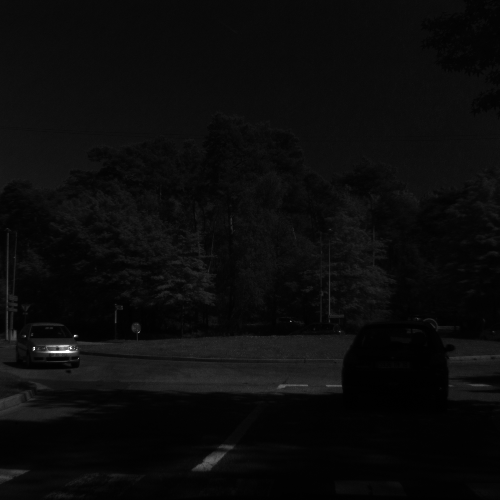
\includegraphics[width=\linewidth]{images/1625_I0.png}
	\end{subfigure}%
	\begin{subfigure}{.2\textwidth}
		\centering
		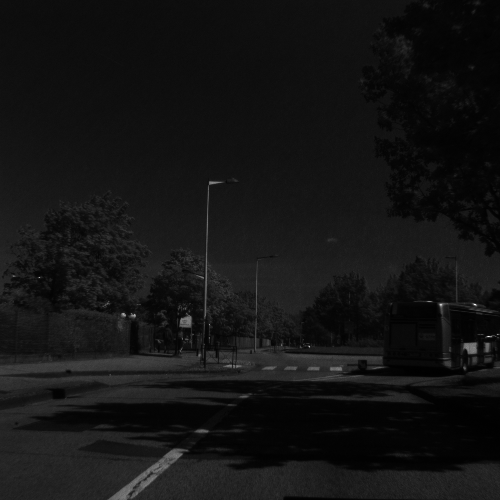
\includegraphics[width=\linewidth]{images/240_I0.png}
	\end{subfigure}%
	\begin{subfigure}{.2\textwidth}
		\centering
		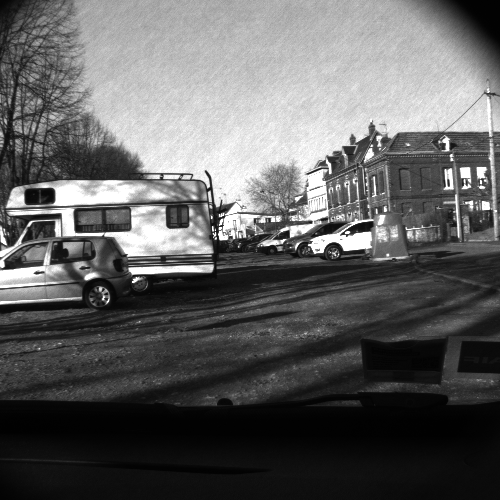
\includegraphics[width=\linewidth]{images/2474_I0.png}
	\end{subfigure}%
	\begin{subfigure}{.2\textwidth}
		\centering
		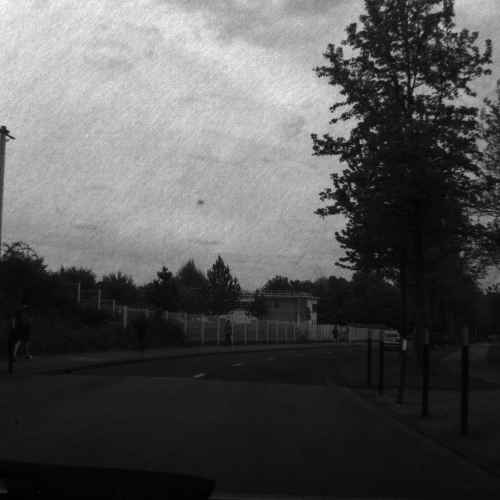
\includegraphics[width=\linewidth]{images/48_I0.png}
	\end{subfigure}%
	\begin{subfigure}{.2\textwidth}
		\centering
		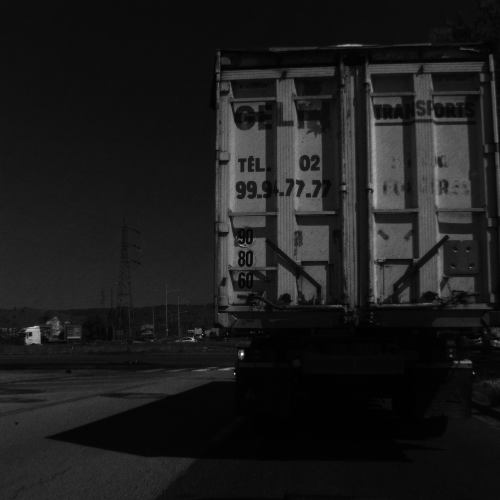
\includegraphics[width=\linewidth]{images/766_I0.png}
	\end{subfigure}
	\caption{Examples of images in the polarimetric dataset \citep{blin2020new}. Only the intensities $I_0$ are shown here.}
	\label{fig:polar_example}
\end{figure}

\begin{figure}
	\centering
	\begin{subfigure}{.2\textwidth}
		\centering
		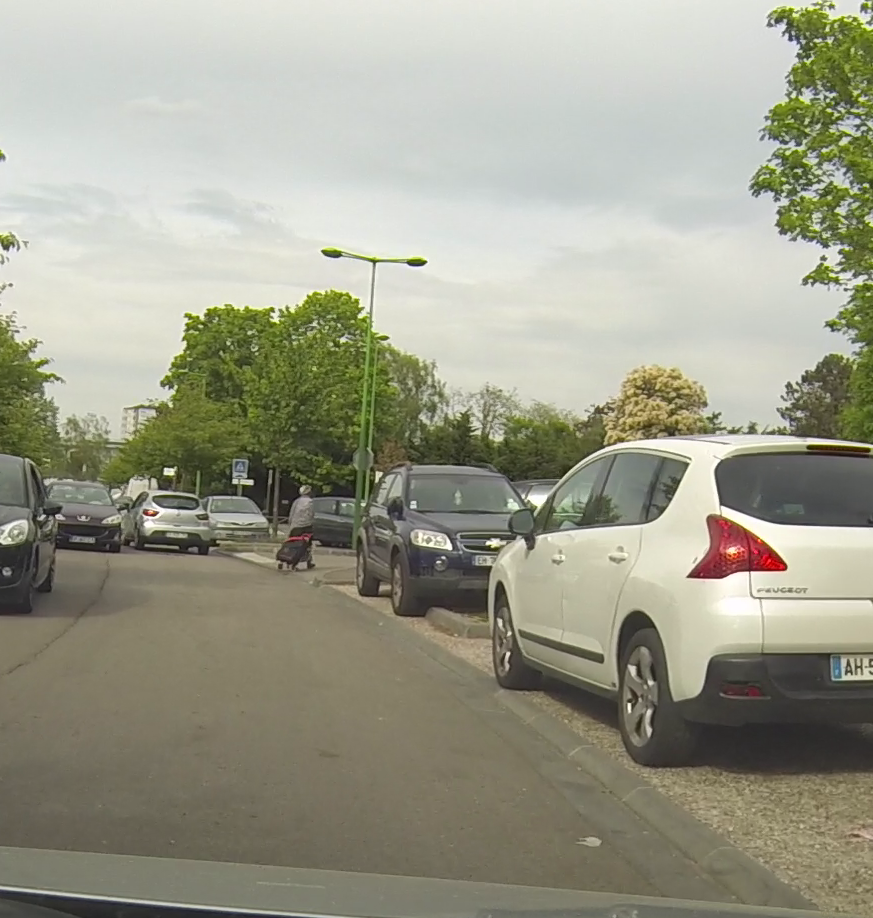
\includegraphics[width=\linewidth]{images/0030144.png}
	\end{subfigure}%
	\begin{subfigure}{.2\textwidth}
		\centering
		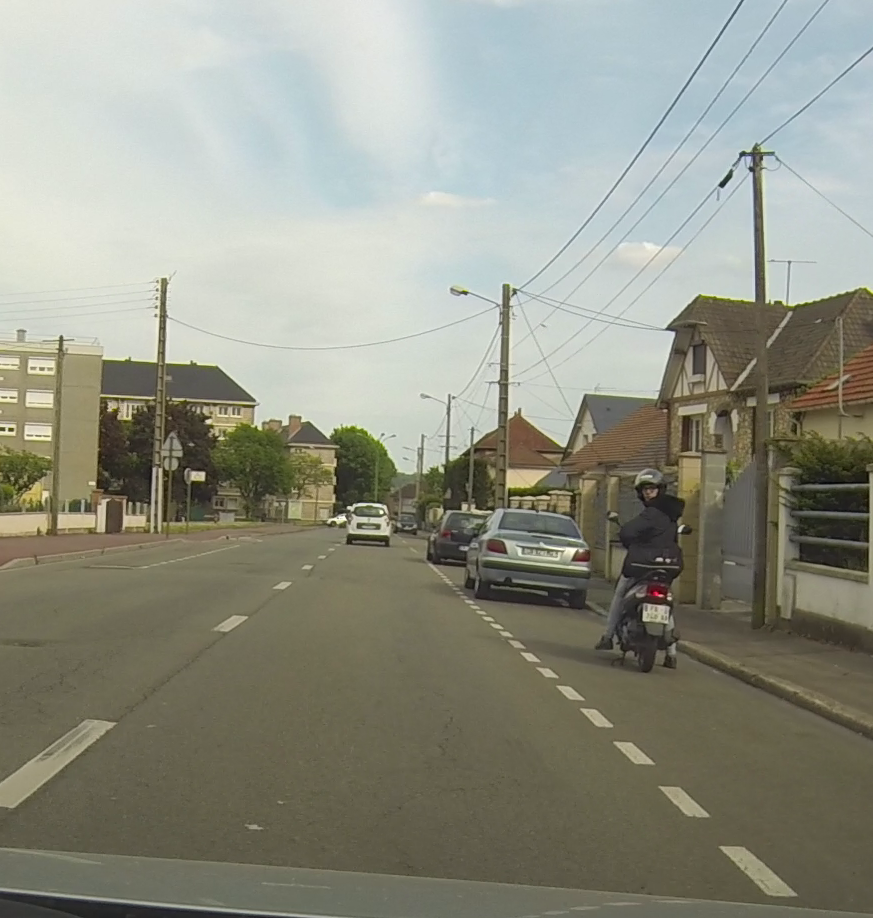
\includegraphics[width=\linewidth]{images/0038544.png}
	\end{subfigure}%
	\begin{subfigure}{.2\textwidth}
		\centering
		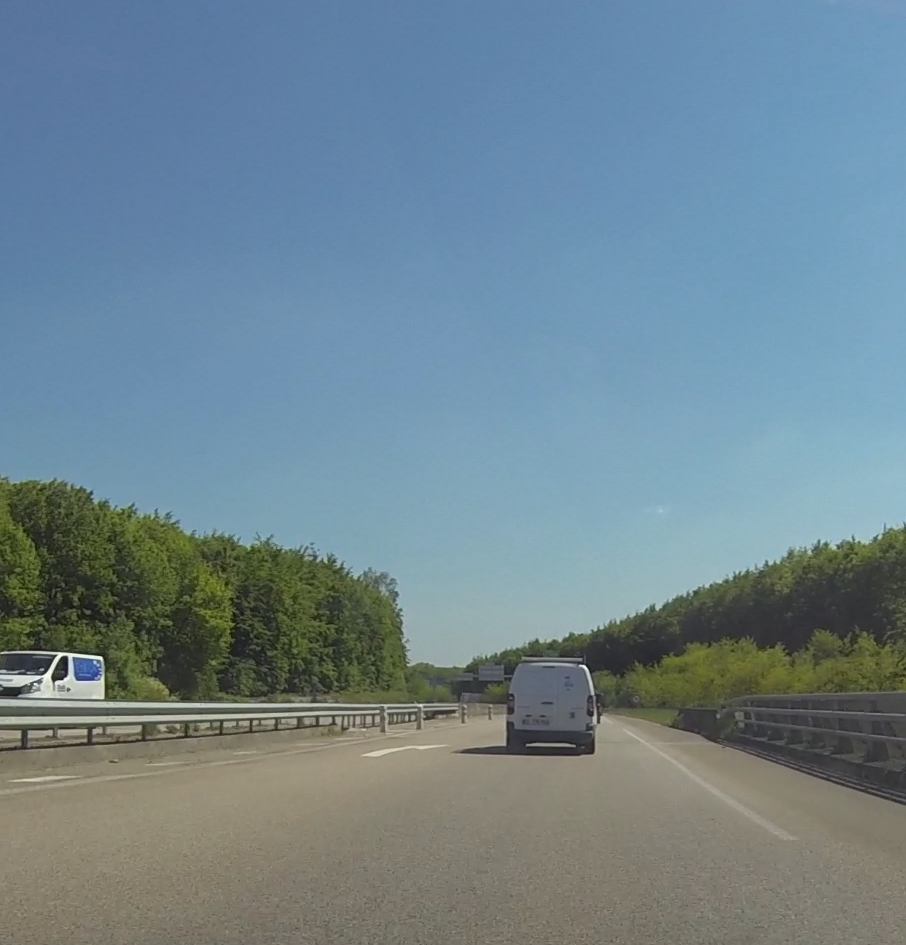
\includegraphics[width=\linewidth]{images/0025879.png}
	\end{subfigure}%
	\begin{subfigure}{.2\textwidth}
		\centering
		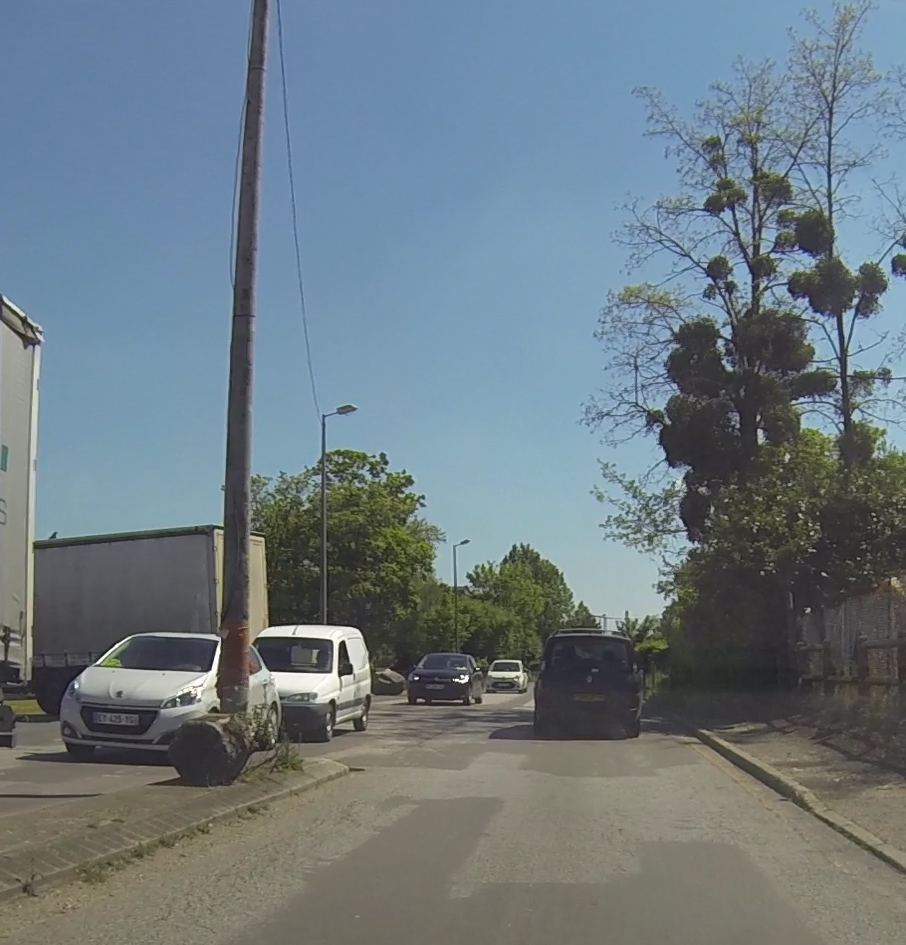
\includegraphics[width=\linewidth]{images/0032059.png}
	\end{subfigure}%
	\begin{subfigure}{.2\textwidth}
		\centering
		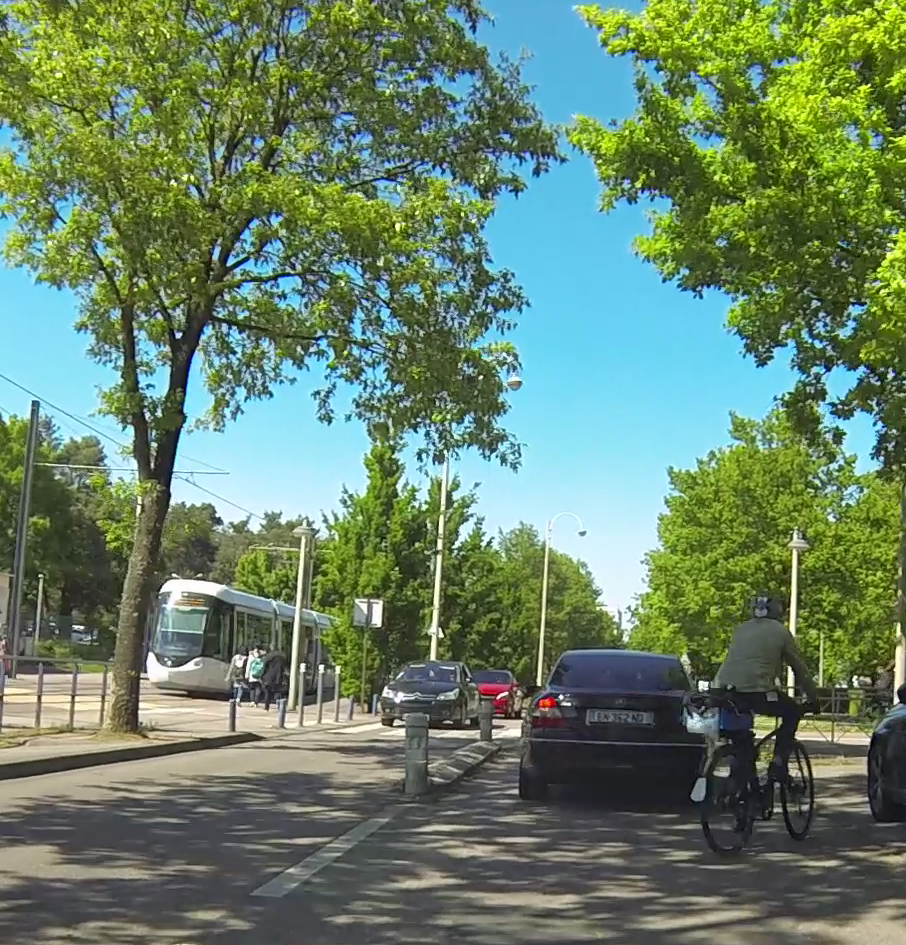
\includegraphics[width=\linewidth]{images/0088999.png}
	\end{subfigure}
	\caption{Examples of images in the RGB dataset.}
	\label{fig:rgb_example}
\end{figure}

Our CycleGAN was trained for 400 epochs on randomly cropped patches of size $200\times 200$. As for the constraints, we found experimentally that setting the hyper-parameters $\mu = 1$ and $\nu = 1$ in equation \eqref{eqn:lfinal} provides the best performances. As for the original CycleGAN, the hyper-parameter $\lambda$, controlling the reconstruction cost,
was set to $\lambda = 10$. The learning rate is decreased linearly from $2 \times 10^{-4}$ to $2 \times 10^{-6}$ during the 400 training epochs.

To evaluate the effectiveness of our trained generative model, we consider KITTI and BDD100K (only using daytime images since polarimetry fails to characterize objects during nighttime) which often serve as testbed in applications related to road scene object detection. The constrained-output CycleGAN we train is used to transfer RGB images from KITTI and BDD100K to the polarimetric domain. The resulting datasets are denoted respectively as Polar-KITTI and Polar-BDD100K. Since the CycleGAN architecture is fully convolutional, it has no requirement on the size of the input image. Therefore, even if the model was trained on $200 \times 200$ patches, it scales straightforwardly to the images of size $1250 \times 375$ from KITTI and of size $1280 \times 720$ from BDD100K datasets.

To assess whether or not fulfilling the physical  constraints is paramount, we investigate a variant of Polar-KITTI and Polar-BDD100K: we learn a standard unconstrained CycleGAN based on the same unpaired RGB/polarimetric images. It is worth mentioning that the so generated polarization-encoded images do not mandatory satisfy the feasibility constraints. 

\subsection{Evaluation of the generated images} \label{subsec:eval_gen_img}
In order to assert the ability of the generated Polar-KITTI and Polar-BDD100K datasets to preserve the relevant features for road scene applications, we train a detection network following the setup in Figure~\ref{fig:experimental_setup}. For this experiment, a RetinaNet-50 \citep{lin2017focal} pre-trained on the MS COCO dataset \citep{lin2014microsoft} is fine-tuned in two different settings. In the first setup the detection model is fine-tuned based on the original RGB KITTI (or BDD100K) while the second experimental setting considers the fine-tuning on the generated polarimetric images from KITTI (Polar-KITTI) or BDD100K (Polar-BDD100K) datasets. Afterwards the final detection models are obtained in both settings by a final fine-tuning on the real polarimetric dataset (see Table \ref{tab:dataset_properties}). The same experiments were carried out for the unconstrained variant of the generated images.

\begin{figure}
	\centering
	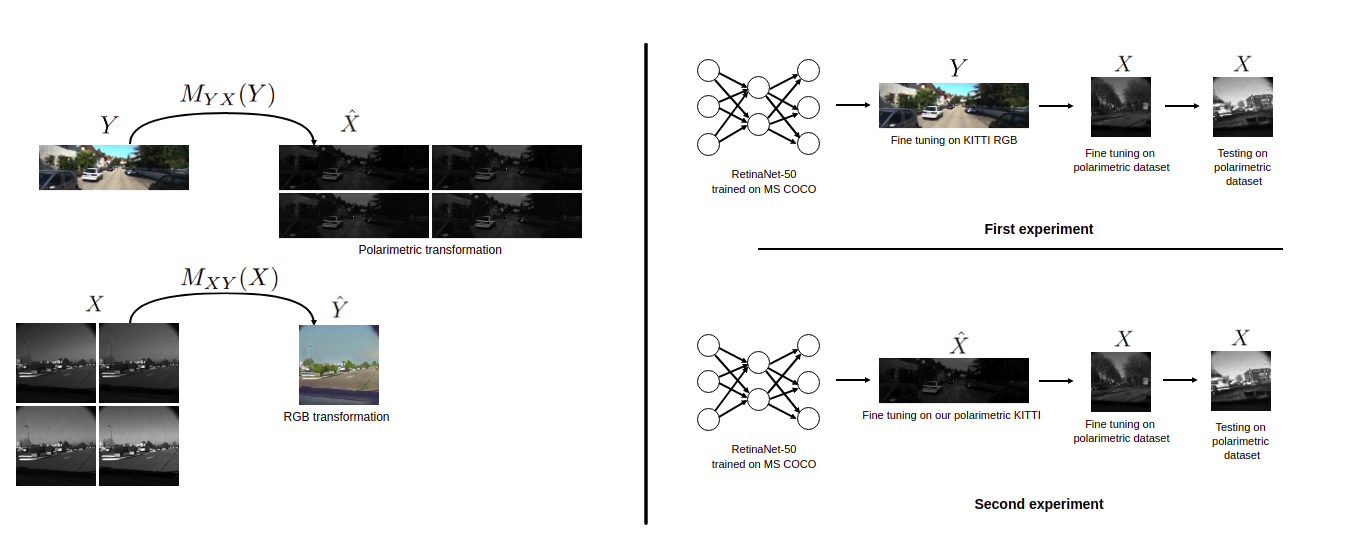
\includegraphics[width=\textwidth]{images/Final_experiment_correction.png}
	\caption{Setup of the detection evaluation experiment. The procedure is illustrated with the KITTI dataset and straightforwardly extends to the BDD100K dataset.}
	\label{fig:experimental_setup}
\end{figure}

Overall, the trained CycleGANs and detection networks under these settings are evaluated in qualitative and quantitative ways. The end goal is to check: (i) the ability of the generated images to help learning polarimetry-based features for object detection, and (ii) the influence of respecting the polarimetric feasibility constraints on detection performances.

We  measure the visual quality of the generated images by computing the classical Fréchet Inception Distance \citep{heusel2017}. Computing this distance requires to extract visual features from each set of images (real and generated) using a pre-trained deep neural network (usually an Inception v3 \citep{szegedy2016} network pre-trained on ImageNet \citep{deng2009imagenet}) and to evaluate the Fréchet (or Wasserstein) distance between the distributions of these features, which are assumed be Gaussian distributions. We calculate this distance using 509 images from each generated polarimetric dataset and from the test set as described in Table \ref{tab:dataset_properties}.

As feature extractor, since the classical Inception v3 network is not adapted to polarimetric images, we use the convolutional part of a polarimetry-adapted RetinaNet detection network \cite{blin2019road}, which has been trained on the MS-COCO dataset and fine-tuned on a real polarimetric dataset.
%
In order to evaluate the improvements in the detection, we compute the error rate evolution $ER_o$. The improvement $ER_o$ on the detection of the object $o$ is given by:
$$
ER_o = \frac{1 - AP_o^{p} - (1 - AP_o^{RGB})}{1-AP_o^{RGB}}\enspace,
$$

\noindent where $AP_o^{RGB}$ and $AP_o^{p}$ respectively denote the average precision for object $o$ detection in RGB and in polarimetric images.

\subsection{Results and discussion}

First we evaluate whether the generated images are qualitatively coherent. For the sake, we reconstruct the polarimetric images from their RGB generation, wich refers to $M_{XY} \circ M_{YX}$ in subsection $2.2$. The reconstruction of these RGB images is shown in Figure~\ref{fig:reco_polar}. 
% A visual comparison of the same generated polarimetric image with and without constraints is illustrated in Figure~\ref{fig:generated_kitti}. As can be seen, the scene content of the generated images is preserved.
%\RB{La Figure 7 est-elle vraiment pertinente en fin de compte? Elle prend beaucoup de place et au final on ne comprend pas ce qu'elle cherche à démontrer}

\begin{figure}
	\centering
	% 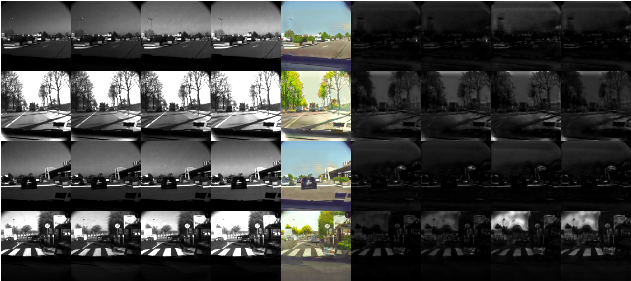
\includegraphics[width=\linewidth]{images/reco_polar.png}
	\begin{subfigure}{.11\textwidth}
		\centering
		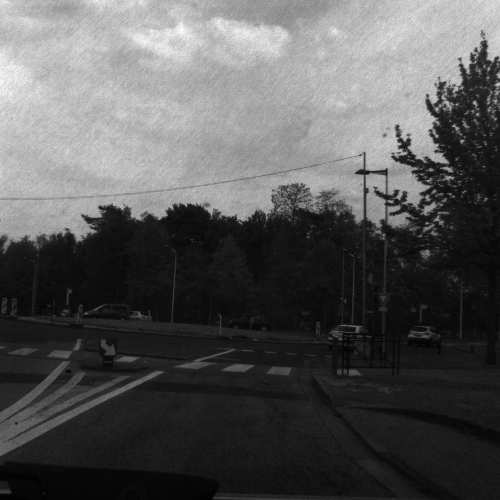
\includegraphics[width=\linewidth]{images/0001611_I0.png}
	\end{subfigure}%
	\begin{subfigure}{.11\textwidth}
		\centering
		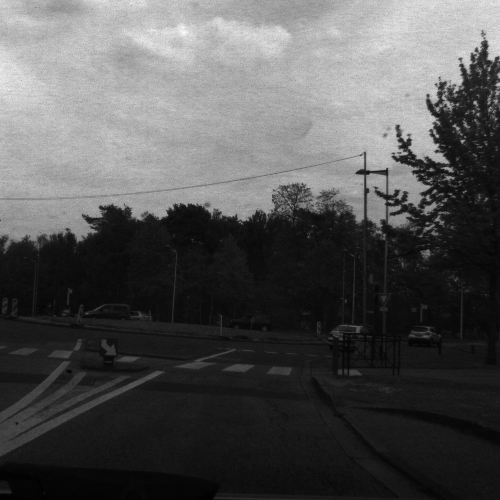
\includegraphics[width=\linewidth]{images/0001611_I45.png}
	\end{subfigure}%
	\begin{subfigure}{.11\textwidth}
		\centering
		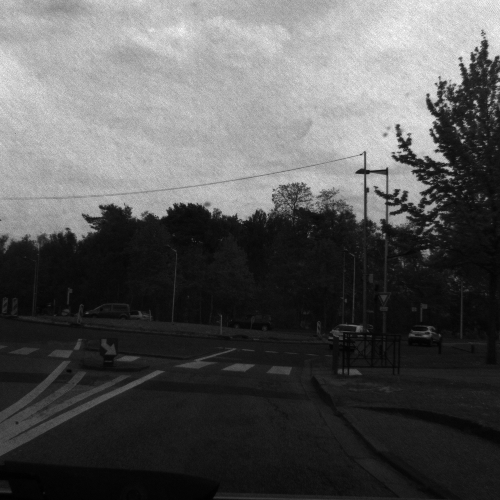
\includegraphics[width=\linewidth]{images/0001611_I90.png}
	\end{subfigure}%
	\begin{subfigure}{.11\textwidth}
		\centering
		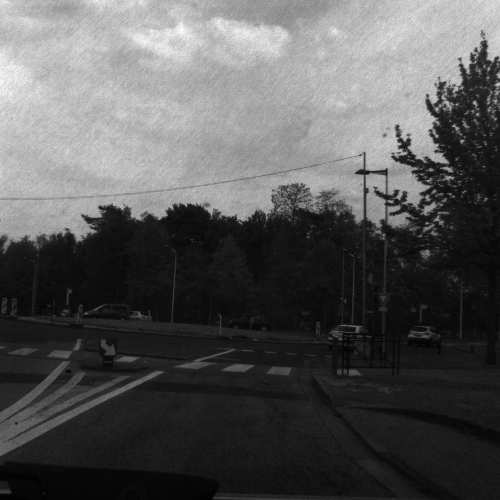
\includegraphics[width=\linewidth]{images/0001611_I0.png}
	\end{subfigure}%
	\begin{subfigure}{.105\textwidth}
		\centering
		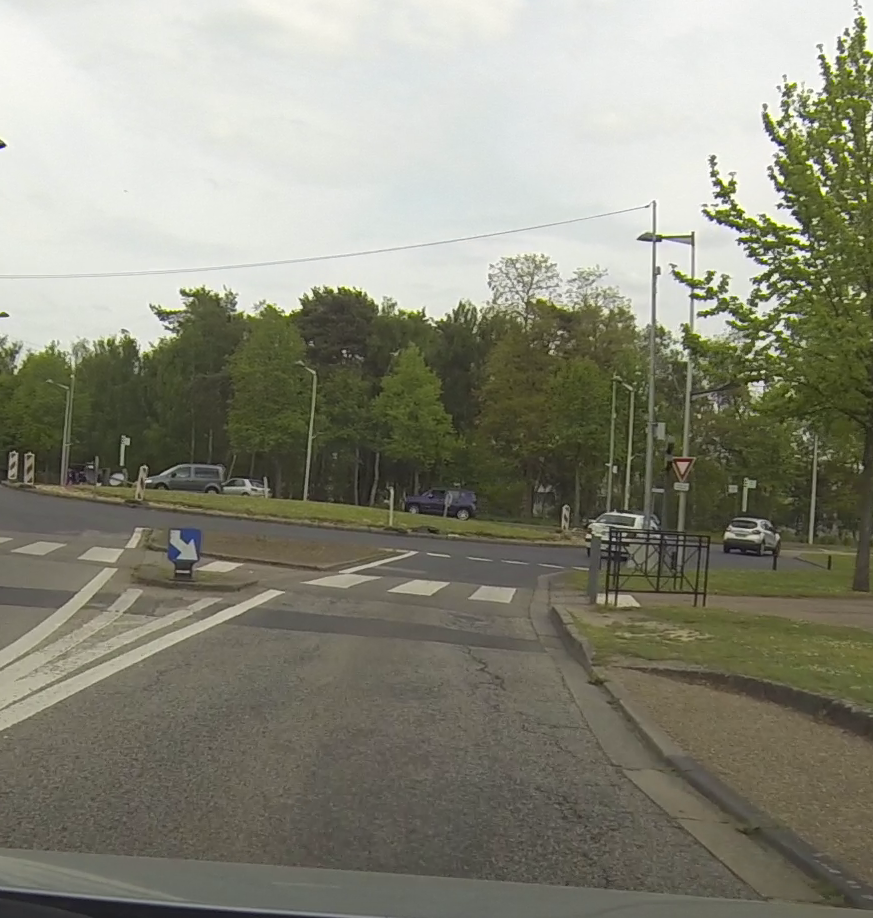
\includegraphics[width=\linewidth]{images/0003024.png}
	\end{subfigure}%
	\begin{subfigure}{.105\textwidth}
		\centering
		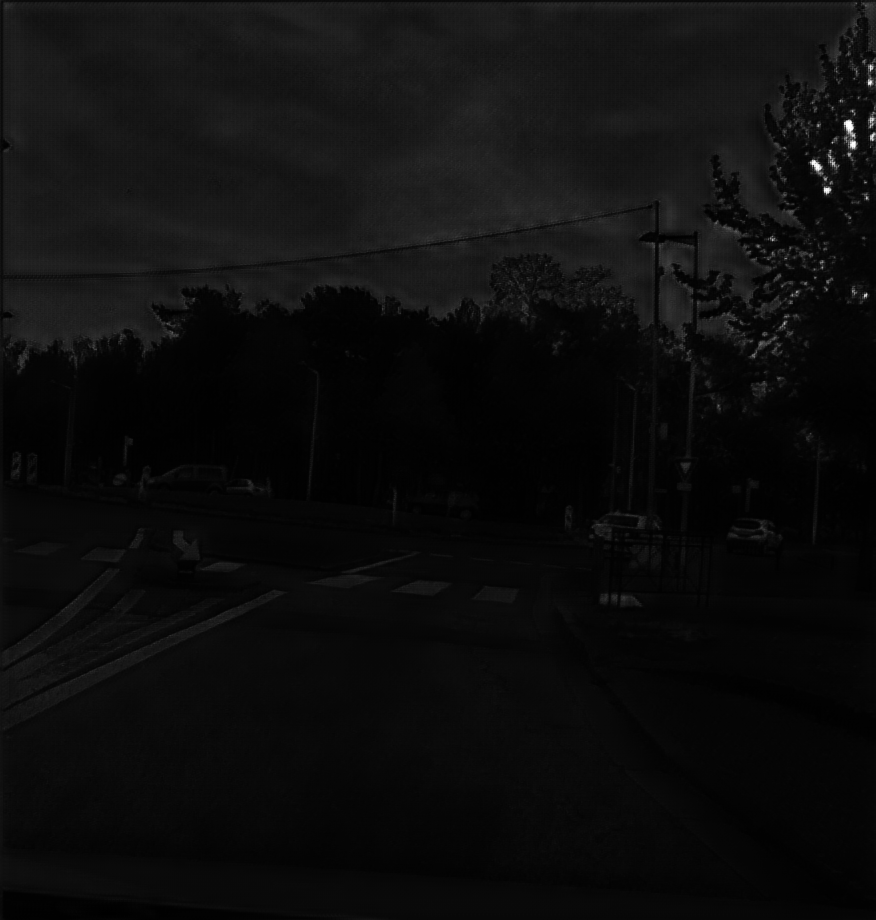
\includegraphics[width=\linewidth]{images/I0_0003024.png}
	\end{subfigure}%
	\begin{subfigure}{.105\textwidth}
		\centering
		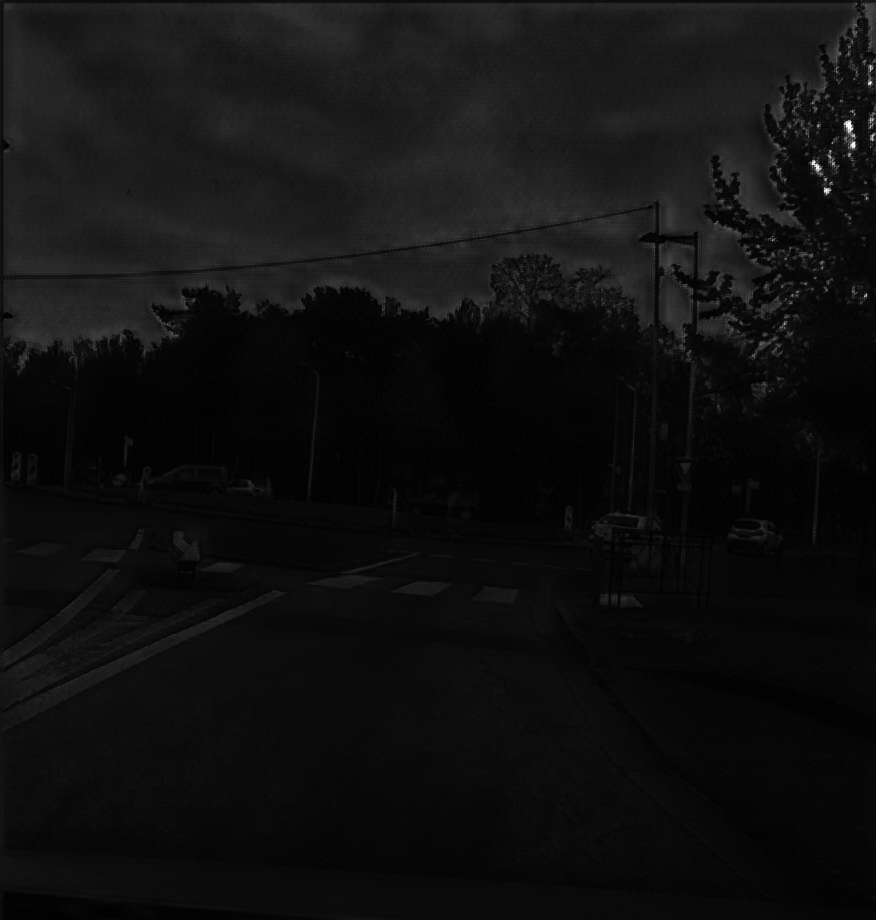
\includegraphics[width=\linewidth]{images/I45_0003024.png}
	\end{subfigure}%
	\begin{subfigure}{.105\textwidth}
		\centering
		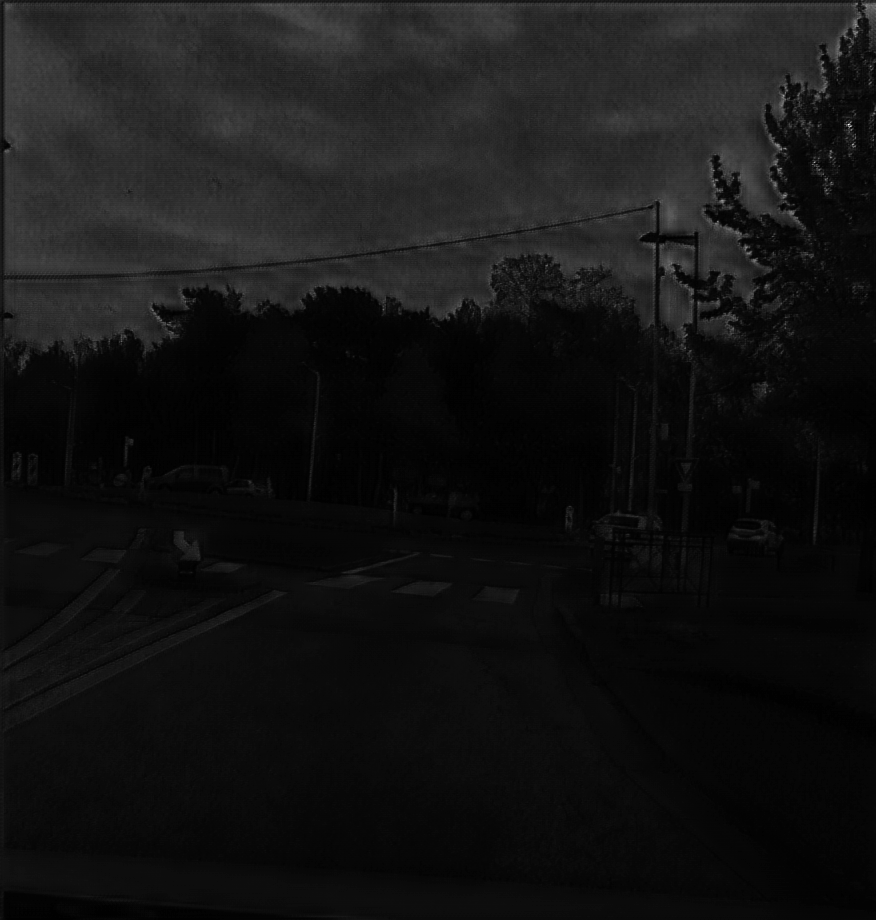
\includegraphics[width=\linewidth]{images/I90_0003024.png}
	\end{subfigure}%
	\begin{subfigure}{.105\textwidth}
		\centering
		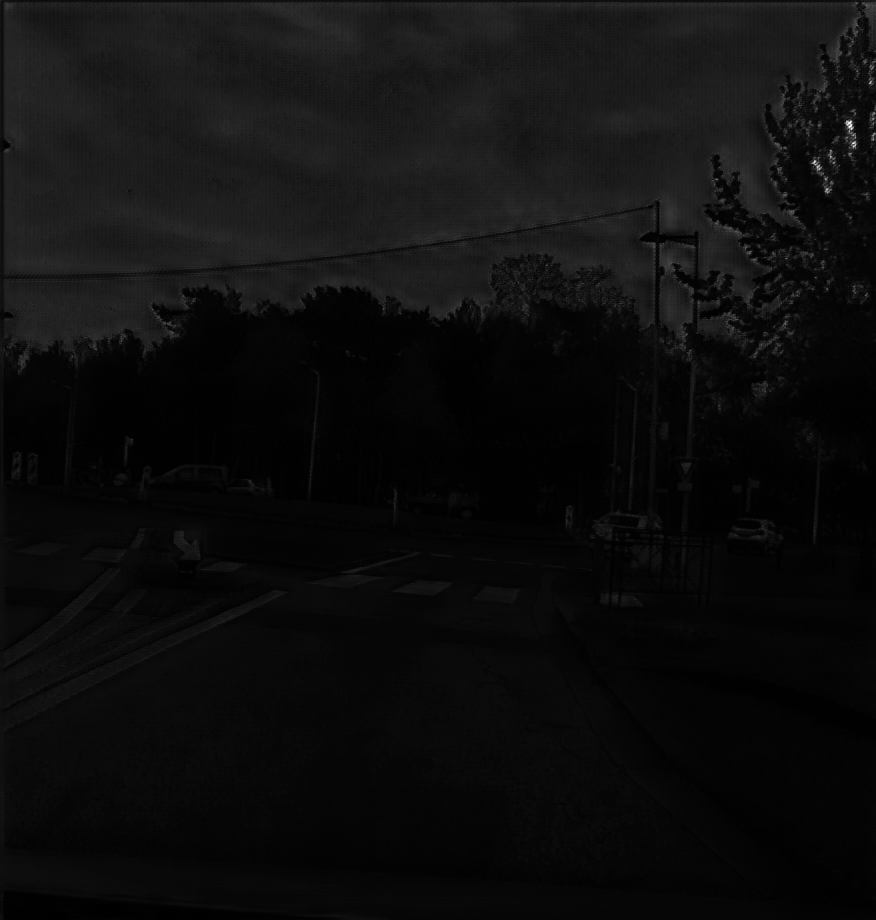
\includegraphics[width=\linewidth]{images/I135_0003024.png}
	\end{subfigure}
	\begin{subfigure}{.11\textwidth}
		\centering
		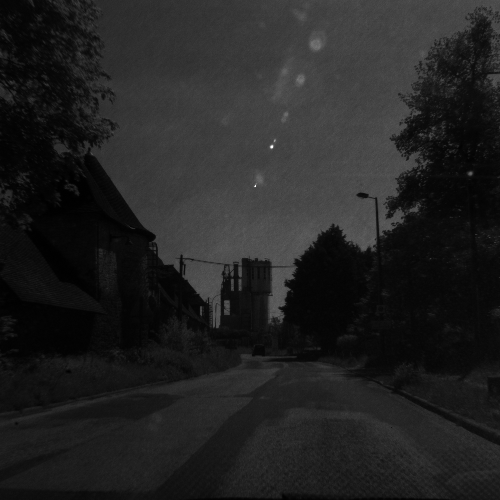
\includegraphics[width=\linewidth]{images/0026648_I0.png}
	\end{subfigure}%
	\begin{subfigure}{.11\textwidth}
		\centering
		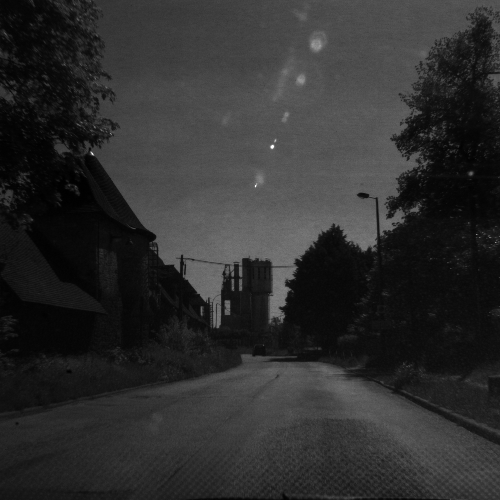
\includegraphics[width=\linewidth]{images/0026648_I45.png}
	\end{subfigure}%
	\begin{subfigure}{.11\textwidth}
		\centering
		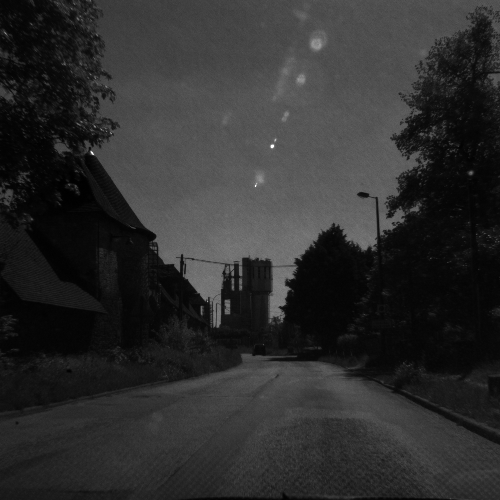
\includegraphics[width=\linewidth]{images/0026648_I90.png}
	\end{subfigure}%
	\begin{subfigure}{.11\textwidth}
		\centering
		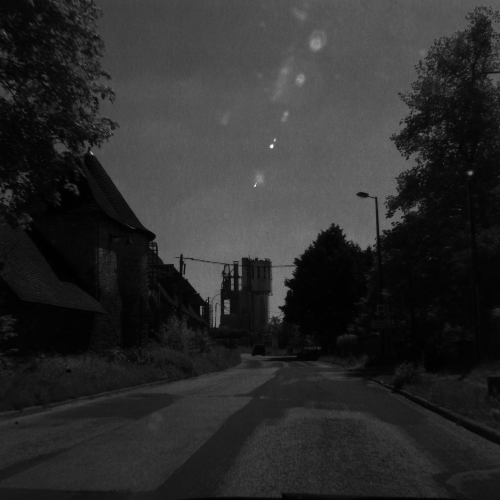
\includegraphics[width=\linewidth]{images/0026648_I135.png}
	\end{subfigure}%
	\begin{subfigure}{.105\textwidth}
		\centering
		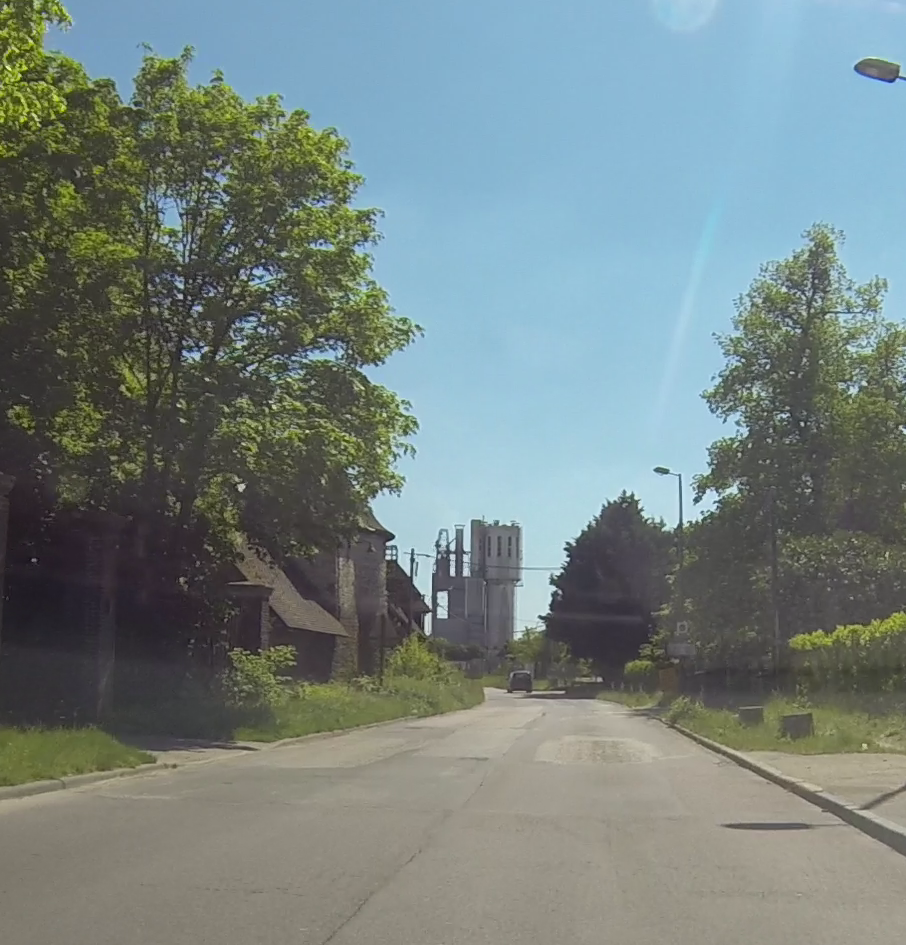
\includegraphics[width=\linewidth]{images/0033019.png}
	\end{subfigure}%
	\begin{subfigure}{.105\textwidth}
		\centering
		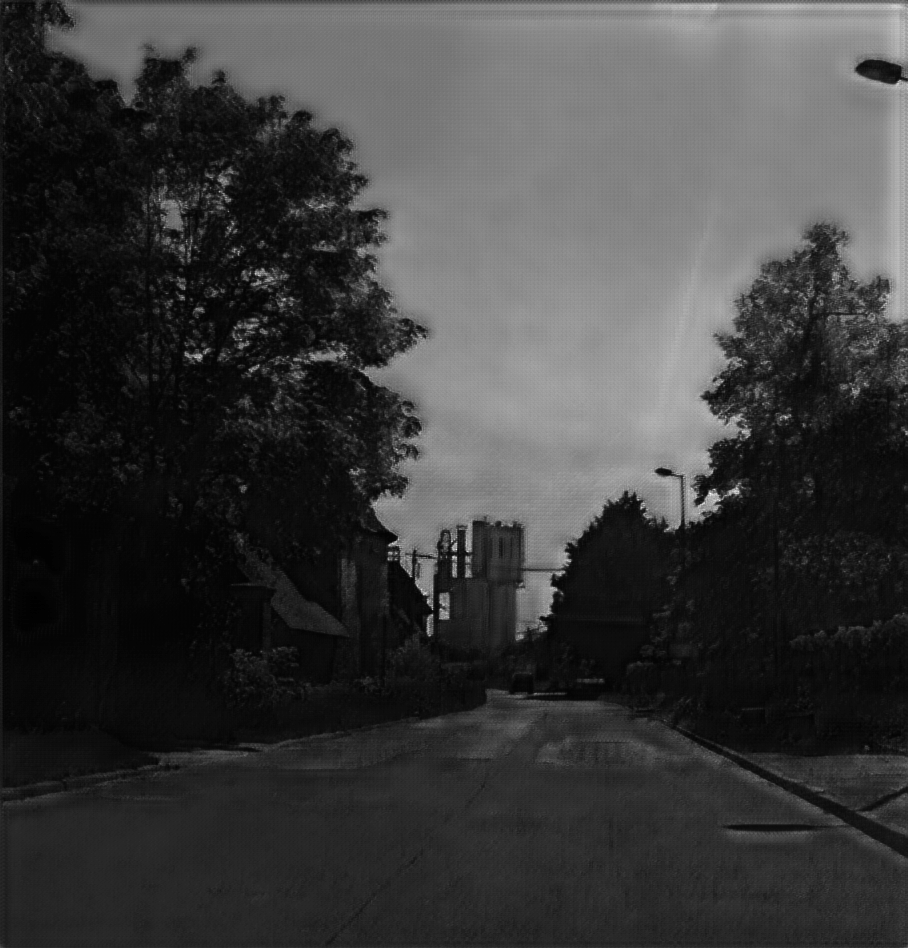
\includegraphics[width=\linewidth]{images/I0_0033019.png}
	\end{subfigure}%
	\begin{subfigure}{.105\textwidth}
		\centering
		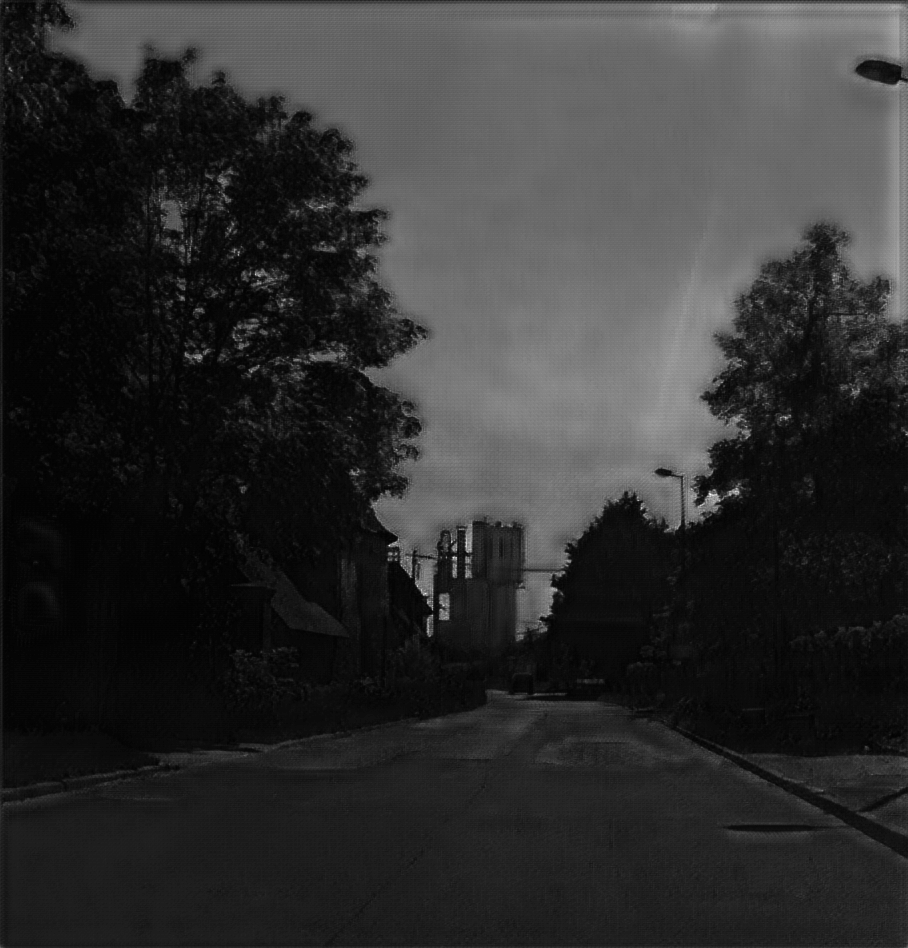
\includegraphics[width=\linewidth]{images/I45_0033019.png}
	\end{subfigure}%
	\begin{subfigure}{.105\textwidth}
		\centering
		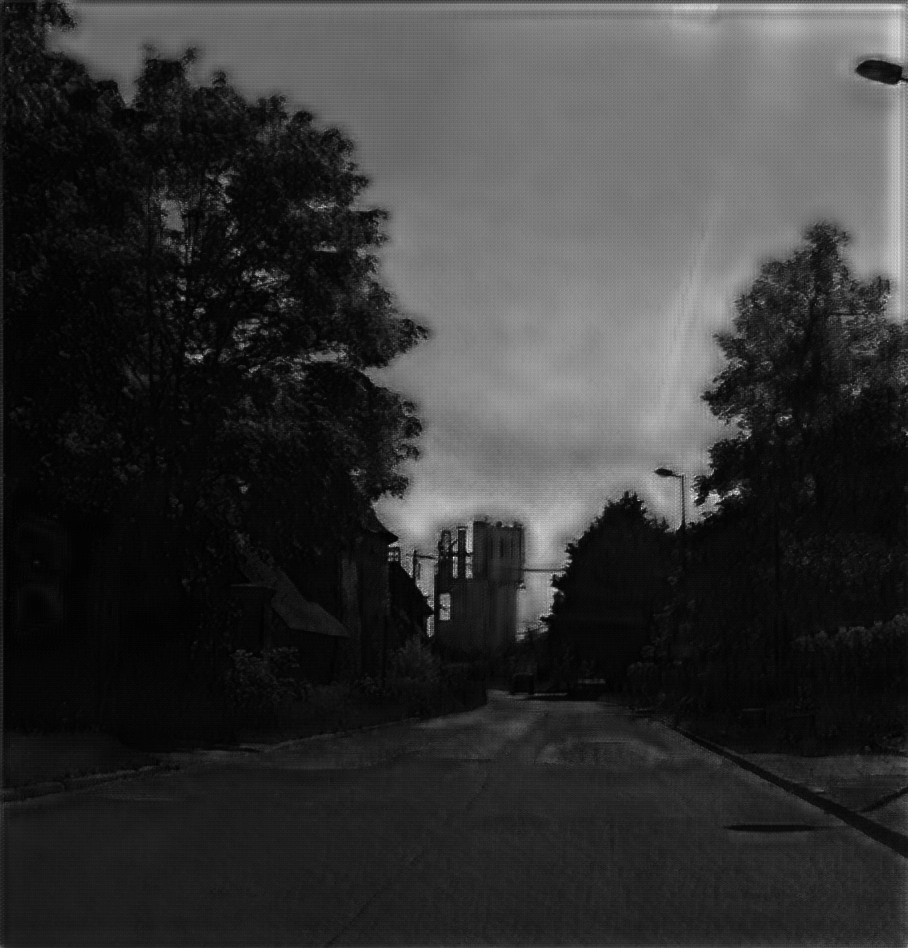
\includegraphics[width=\linewidth]{images/I90_0033019.png}
	\end{subfigure}%
	\begin{subfigure}{.105\textwidth}
		\centering
		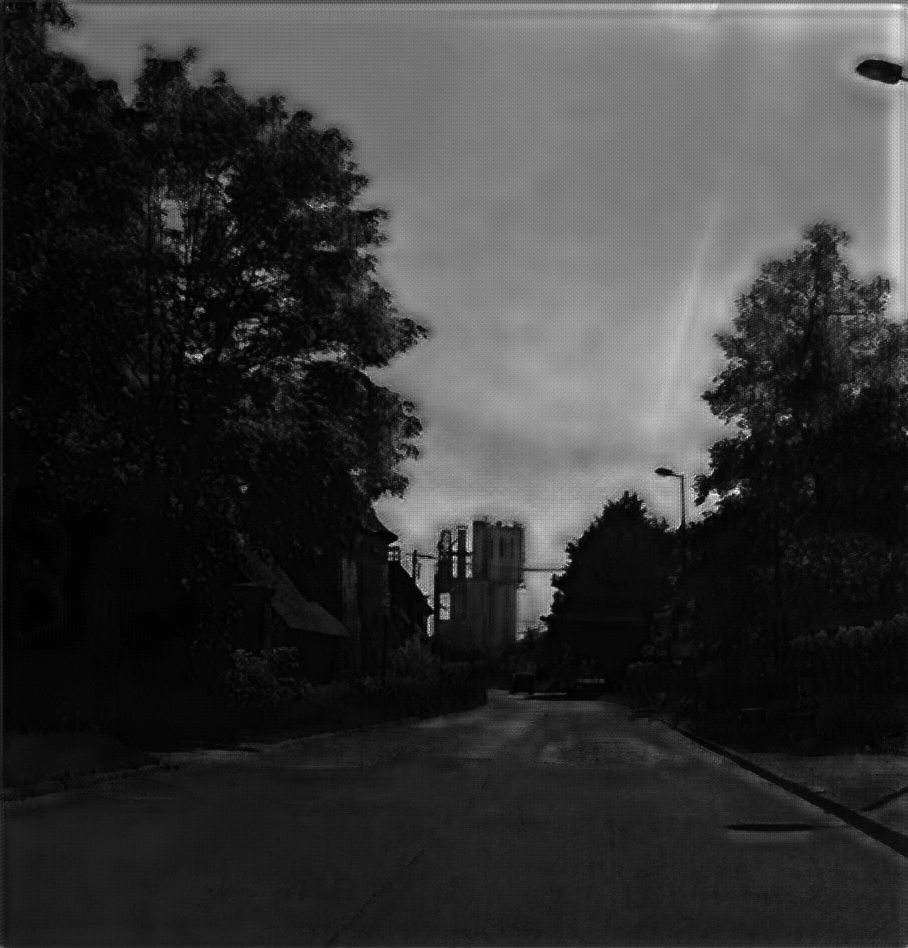
\includegraphics[width=\linewidth]{images/I135_0033019.png}
	\end{subfigure}
	\begin{subfigure}{.11\textwidth}
		\centering
		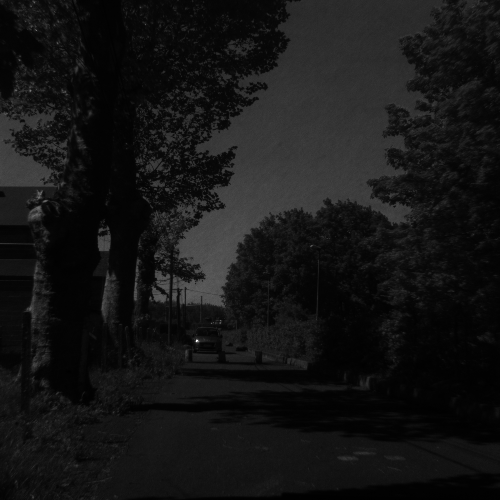
\includegraphics[width=\linewidth]{images/0033248_I0.png}
	\end{subfigure}%
	\begin{subfigure}{.11\textwidth}
		\centering
		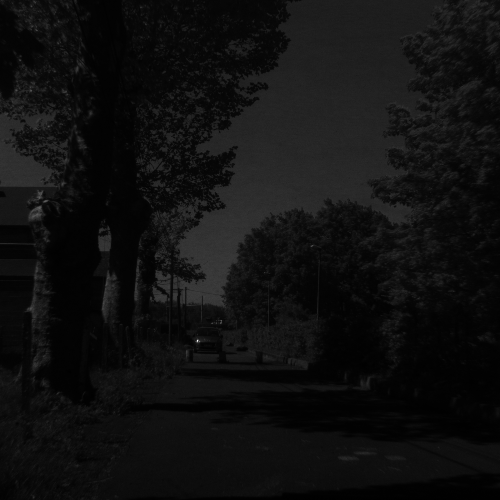
\includegraphics[width=\linewidth]{images/0033248_I45.png}
	\end{subfigure}%
	\begin{subfigure}{.11\textwidth}
		\centering
		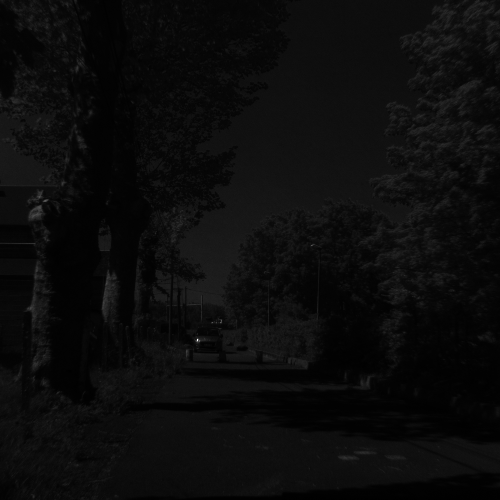
\includegraphics[width=\linewidth]{images/0033248_I90.png}
	\end{subfigure}%
	\begin{subfigure}{.11\textwidth}
		\centering
		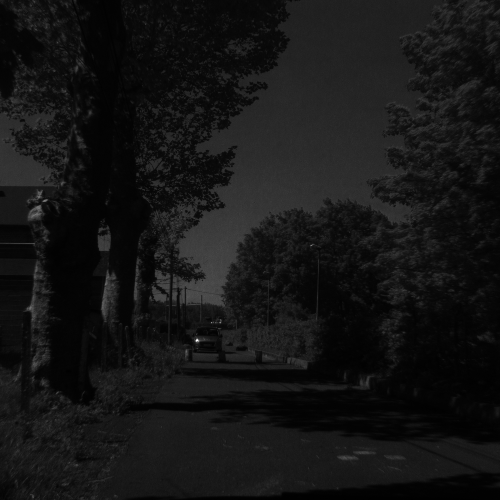
\includegraphics[width=\linewidth]{images/0033248_I135.png}
	\end{subfigure}%
	\begin{subfigure}{.105\textwidth}
		\centering
		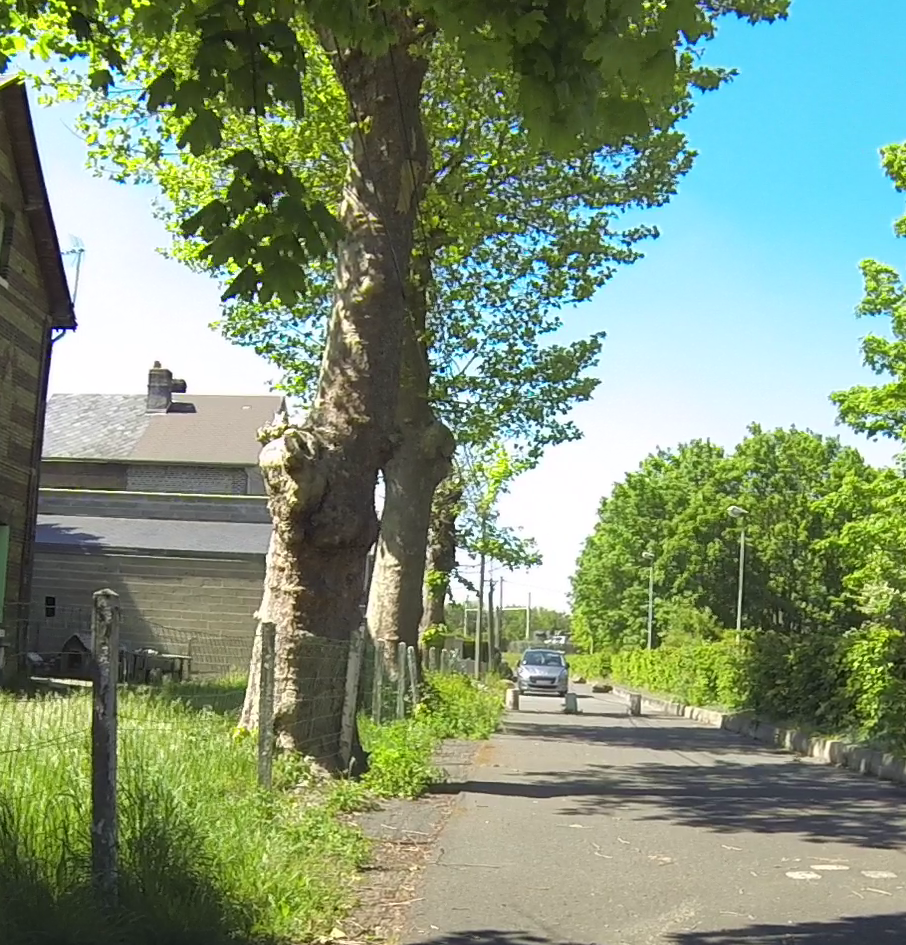
\includegraphics[width=\linewidth]{images/0040999.png}
	\end{subfigure}%
	\begin{subfigure}{.105\textwidth}
		\centering
		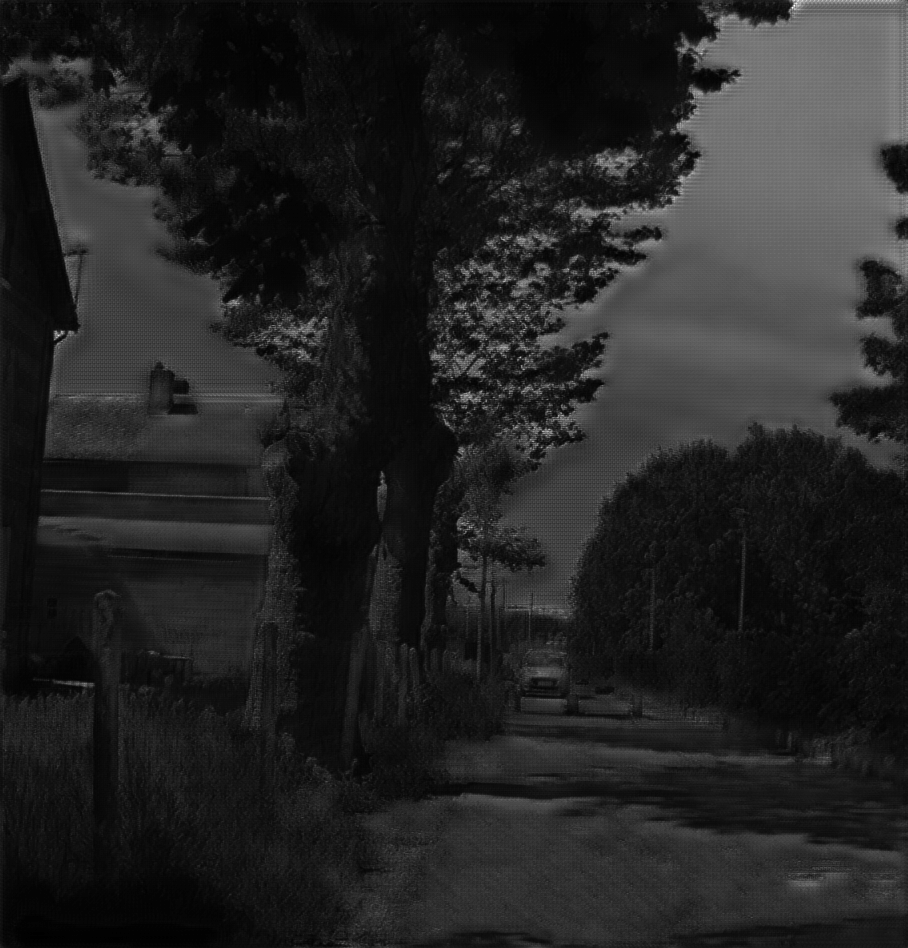
\includegraphics[width=\linewidth]{images/I0_0040999.png}
	\end{subfigure}%
	\begin{subfigure}{.105\textwidth}
		\centering
		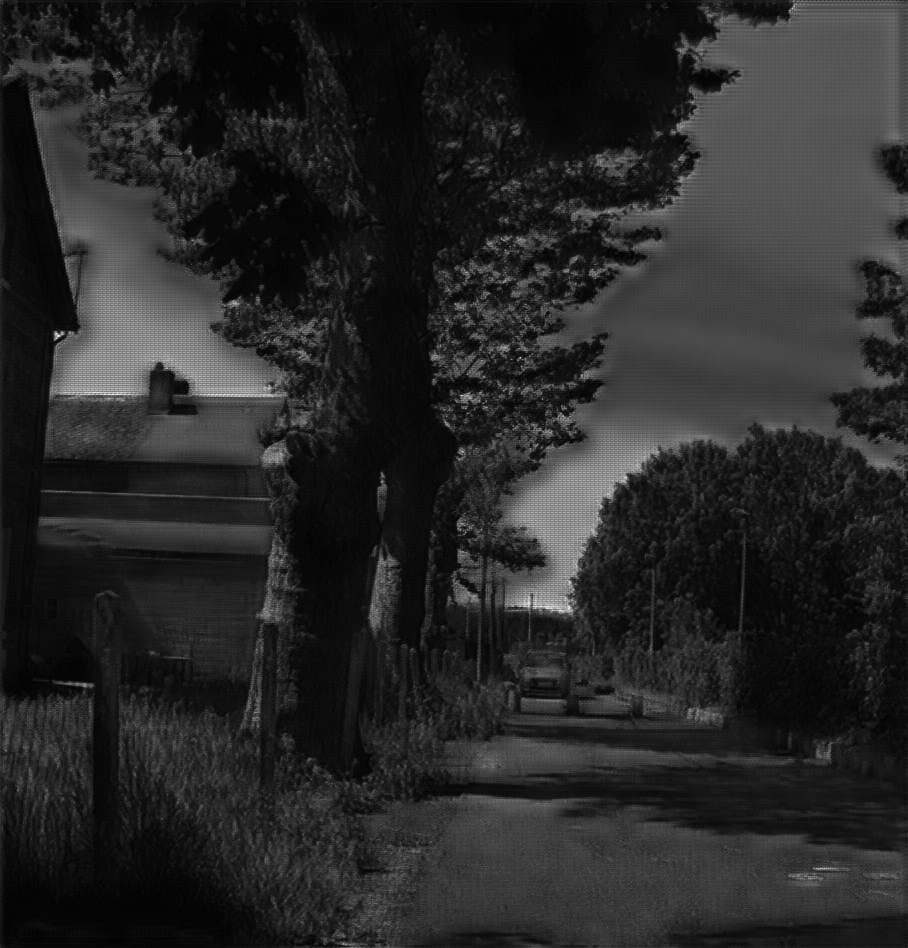
\includegraphics[width=\linewidth]{images/I45_0040999.png}
	\end{subfigure}%
	\begin{subfigure}{.105\textwidth}
		\centering
		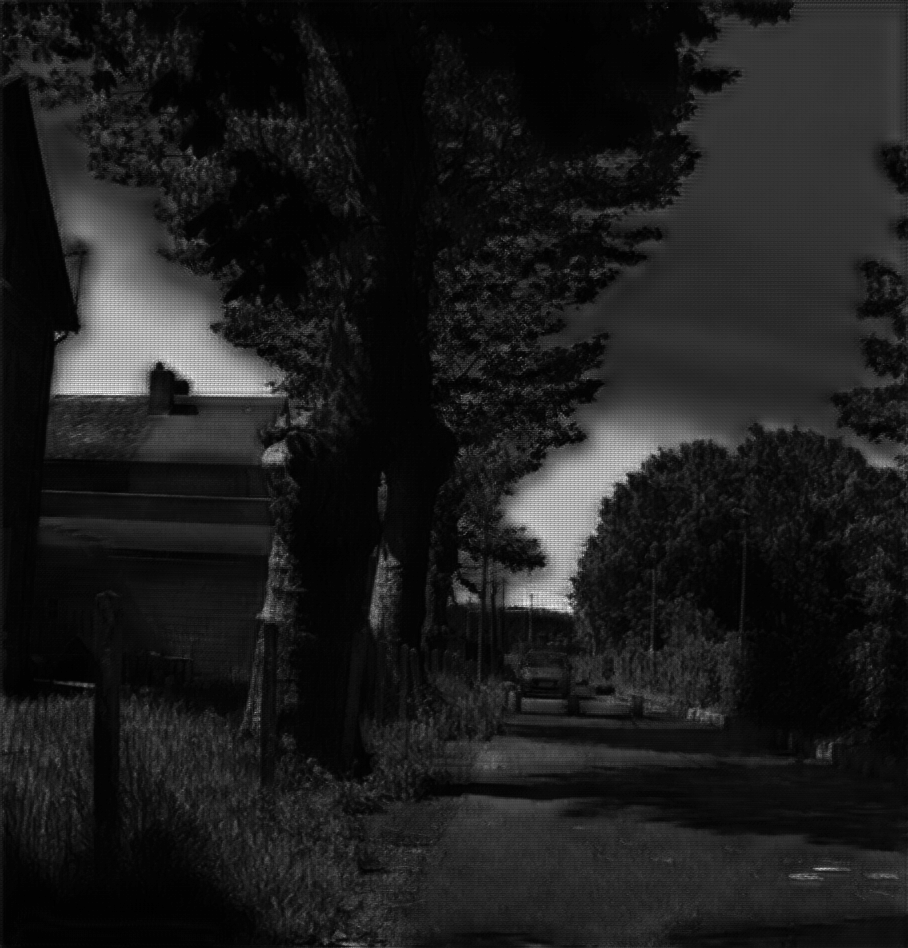
\includegraphics[width=\linewidth]{images/I90_0040999.png}
	\end{subfigure}%
	\begin{subfigure}{.105\textwidth}
		\centering
		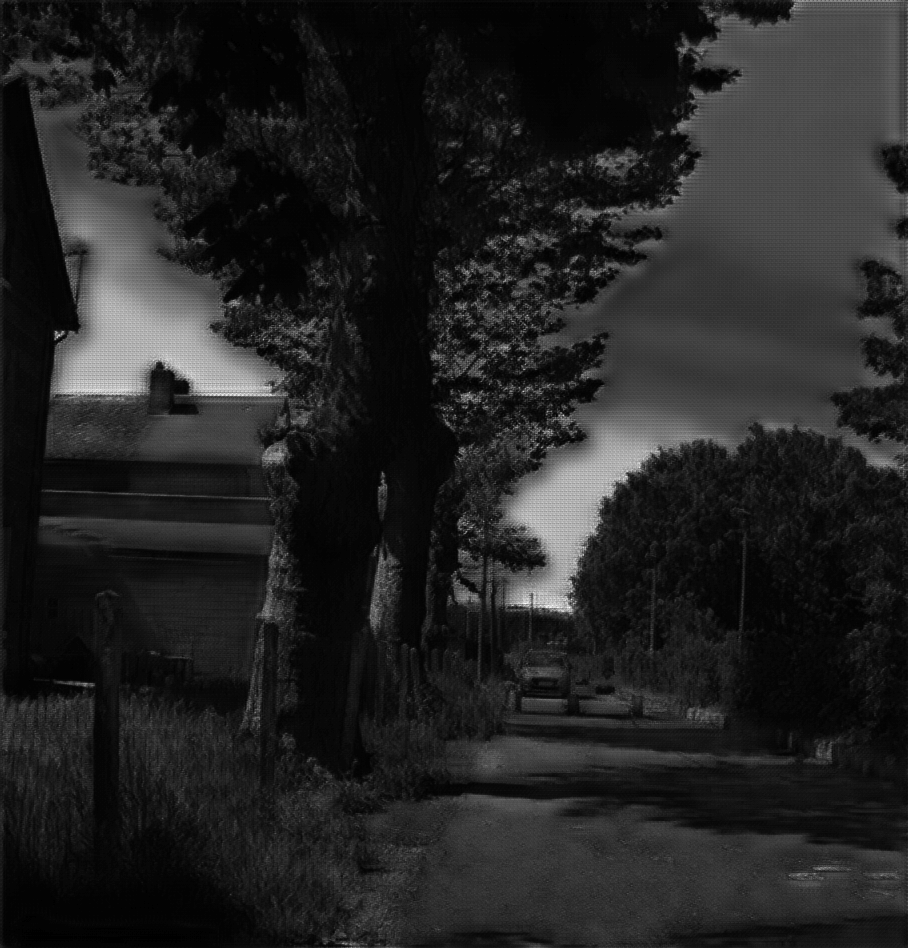
\includegraphics[width=\linewidth]{images/I135_0040999.png}
	\end{subfigure}
	\begin{subfigure}{.11\textwidth}
		\centering
		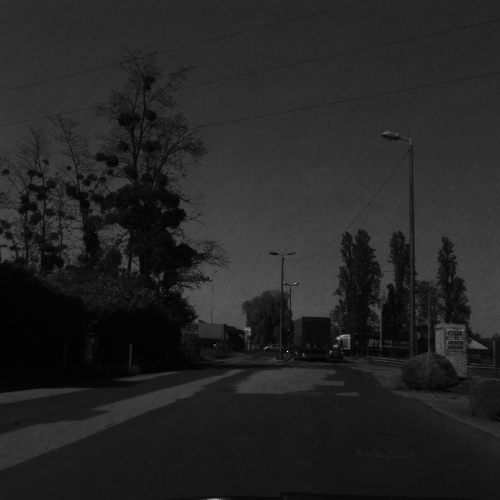
\includegraphics[width=\linewidth]{images/0048448_I0.png}
	\end{subfigure}%
	\begin{subfigure}{.11\textwidth}
		\centering
		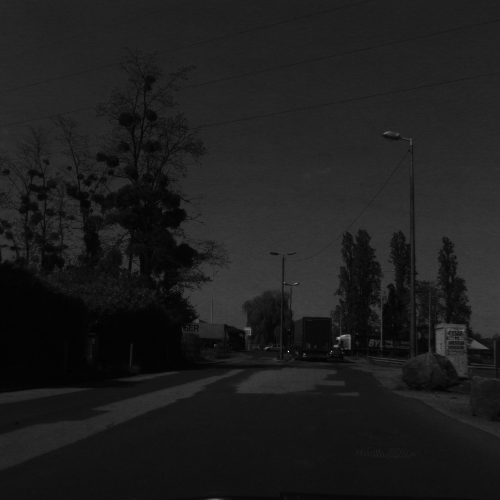
\includegraphics[width=\linewidth]{images/0048448_I45.png}
	\end{subfigure}%
	\begin{subfigure}{.11\textwidth}
		\centering
		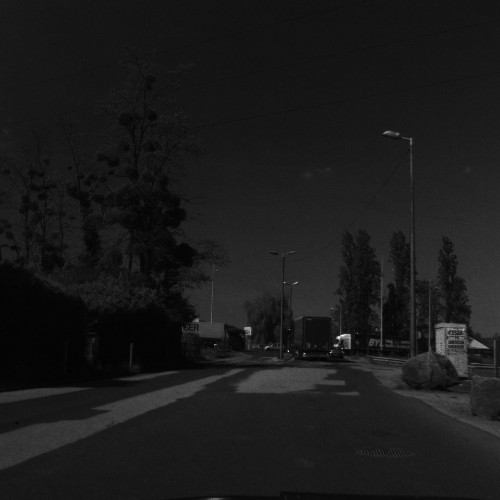
\includegraphics[width=\linewidth]{images/0048448_I90.png}
	\end{subfigure}%
	\begin{subfigure}{.11\textwidth}
		\centering
		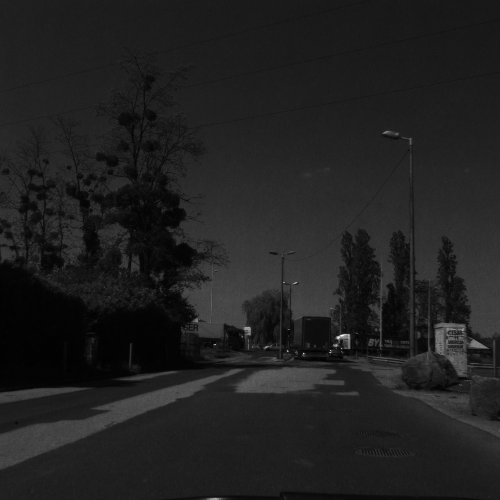
\includegraphics[width=\linewidth]{images/0048448_I135.png}
	\end{subfigure}%
	\begin{subfigure}{.105\textwidth}
		\centering
		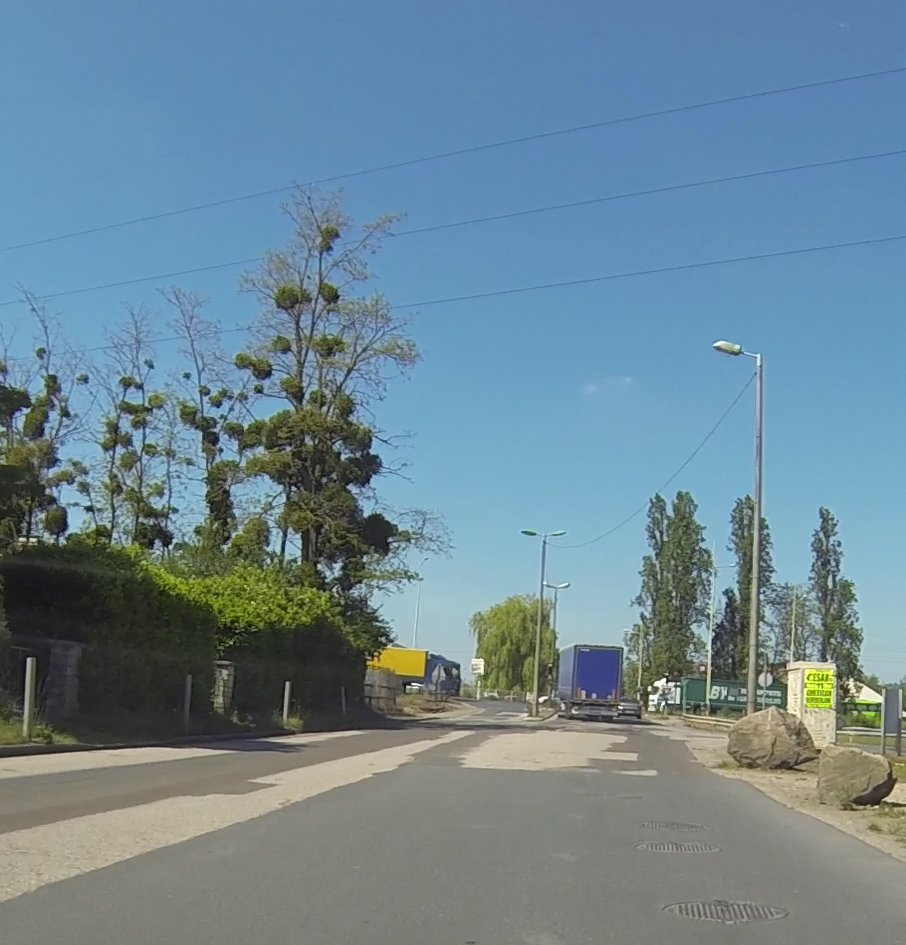
\includegraphics[width=\linewidth]{images/0059179.png}
	\end{subfigure}%
	\begin{subfigure}{.105\textwidth}
		\centering
		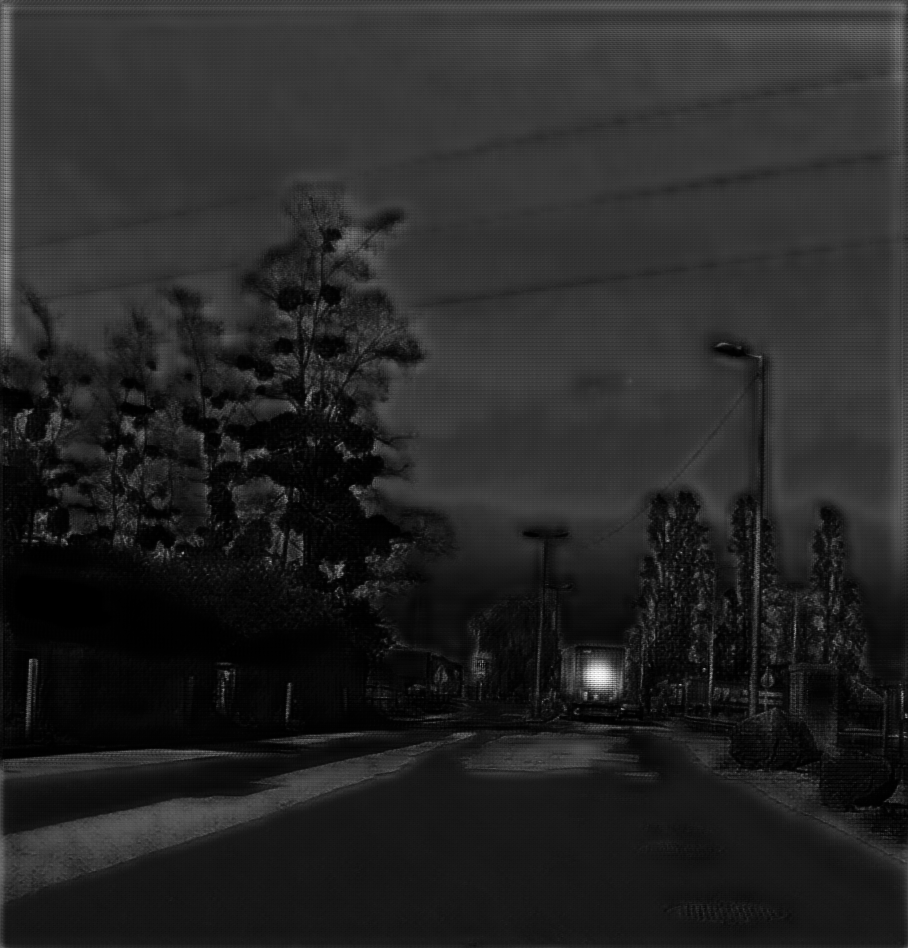
\includegraphics[width=\linewidth]{images/I0_0059179.png}
	\end{subfigure}%
	\begin{subfigure}{.105\textwidth}
		\centering
		\includegraphics[width=\linewidth]{images/I45_0059179.png}
	\end{subfigure}%
	\begin{subfigure}{.105\textwidth}
		\centering
		\includegraphics[width=\linewidth]{images/I90_0059179.png}
	\end{subfigure}%
	\begin{subfigure}{.105\textwidth}
		\centering
		\includegraphics[width=\linewidth]{images/I135_0059179.png}
	\end{subfigure}
	\caption{Examples  of polarimetric image reconstruction. From left to right: $I_0$, $I_{45}$, $I_{90}$ and $I_{135}$ ground truth, RGB image and $I_0$, $I_{45}$, $I_{90}$ and $I_{135}$ generated from RGB image.}
	\label{fig:reco_polar}
\end{figure}

% \begin{figure}
%     \centering
%     \includegraphics[width=\linewidth]{images/comparison_generation.png}
%     \caption{Example of generated images (Polar-KITTI). The left column represents the generation with constraints and the right column refers to image generation without constraints. From top to bottom: $I_0$, $I_{45}$, $I_{90}$ and $I_{135}$.}
%     \label{fig:generated_kitti}
% \end{figure}

As for the constraints, Table \ref{tab:polar_constraints} shows how including them to the CycleGAN's loss helps generating images which better fulfill the physical polarimetric properties at the pixel scale. The errors related to the constraints $\mathcal{C}_1$ and $\mathcal{C}_2$ on generated images using our approach are consistent with the observed errors on the real images, whereas the unconstrained approach yields poor results. Obviously, constraint $\mathcal{C}_3$ is met for all generated images thanks to the tanh activation at the last layer of the generative models. Additionally, the obtained Fréchet Inception Distances are of \textbf{6022.7} for the unconstrained CycleGAN and \textbf{4485.1} for our approach\footnote{Note that the scale of the FID scores computed with the pre-trained RetinaNet is larger than when using a pre-trained Inception v3 network.}, which indicates that taking the constraints into account improves visual and physical quality of the generated samples.

\begin{table}
	\begin{center}
		\begin{tabular}{c c c c}
			\specialrule{.3em}{.2em}{.2em}
			Datasets & $\mathcal{C}$ & Mean & Median \\
			\specialrule{.3em}{.2em}{.2em}
			Real & $\mathcal{C}_1$ & 0.06 $\pm$ 0.04 & 0.04 \\
			polar & $\mathcal{C}_2$ & 2.47 $\pm$ 7.11\% & 0.48\% \\
			& $\mathcal{C}_3$ & 0\% & 0\% \\
			\specialrule{.2em}{.1em}{.1em} 
			Generated & $\mathcal{C}_1$ & 0.26 $\pm$ 0.19 & 0.23 \\
			polar no $\mathcal{C}$ & $\mathcal{C}_2$ & 27.31 $\pm$ 43.5\% & 2.15\% \\
			& $\mathcal{C}_3$ & 0\% & 0\% \\
			\specialrule{.2em}{.1em}{.1em} 
			Generated & $\mathcal{C}_1$ & 0.12 $\pm$ 0.04 & 0.12 \\
			polar with $\mathcal{C}$ & $\mathcal{C}_2$ & 1.55 $\pm$ 3.36\% & 0.14\% \\
			& $\mathcal{C}_3$ & 0\% & 0\% \\
		\end{tabular}
		\caption{Evaluation of the constraint fulfillment using the designed losses $L_{\mathcal{C}_1}$ and $L_{\mathcal{C}_2}$ at the pixel scale. Here, the column $\mathcal{C}$ indicates the evaluated constraint. $\mathcal{C}_1$ refers to the constraints $I = AS$, $\mathcal{C}_2$ to $S_0^2 \geqslant S_1^2 + S_2^2$ and $\mathcal{C}_3$ to $S_0 > 0$. The mean and the median of the percentage of pixels in an image that do not fulfill the constraints $\mathcal{C}_2$ and $\mathcal{C}_3$ are computed. Regarding the constraint $\mathcal{C}_1$, we compute the mean and the median of $||I - AS|| / (||I|| + ||AS||)$.}
		\label{tab:polar_constraints}
	\end{center}
\end{table}

Next, we show the benefit of the generated images in object detection task, enabling to verify that objects in them are globally physically coherent. 
The RetinaNet-based detection model were trained according to the setups described in Section \ref{subsec:eval_gen_img} and the obtained detection performances in term of mean average precision ($mAP$) are summarized in Table \ref{tab:obtained_results}. We choose not to evaluate the bike and motorbike detection performances as the polarimetric dataset does not contain enough objects of those two classes.

\begin{table}
	\begin{center}
		\begin{tabular}{c c c c| c c cc}
			\specialrule{.3em}{.2em}{.2em}
			Databases used & Class & Test & $ER_o$ & Databases used & Class & Test & $ER_o$ \\
			\specialrule{.3em}{.2em}{.2em}
			KITTI RGB & person & 0.663 & N/A & BDD100K RGB & person & 0.736 & N/A \\
			+ real polar & car & 0.785 & N/A & + real polar & car & \textbf{0.821} & N/A \\
			\multicolumn{2}{c}{$mAP$} & 0.724 & N/A & \multicolumn{2}{c}{$mAP$} & 0.778 & N/A \\
			\specialrule{.2em}{.1em}{.1em} 
			Polar-KITTI no $\mathcal{C}$ & person & 0.673 & -0.03 & Polar-BDD100K no $\mathcal{C}$ & person & 0.720 & 0.06 \\
			+ real polar & car & 0.786 & -0.01 & + real polar & car & 0.816 & 0.03 \\
			\multicolumn{2}{c}{$mAP$} & 0.730 & -0.02 & \multicolumn{2}{c}{$mAP$} & 0.768 & 0.05 \\
			\specialrule{.2em}{.1em}{.1em} 
			Polar-KITTI with $\mathcal{C}$ & person & \textbf{0.704} & -0.12 & Polar-BDD100K with $\mathcal{C}$ & person & \textbf{0.762} & -0.10 \\
			+ real polar & car & \textbf{0.794} & -0.04 & + real polar & car & 0.815 & 0.03 \\
			\multicolumn{2}{c}{$mAP$} & \textbf{0.749} & -0.09 & \multicolumn{2}{c}{$mAP$} & \textbf{0.789} & -0.05 \\
		\end{tabular}
	\end{center}
	\caption{
		Comparison of the detection performance after the two successive fine-tunings. RetinaNet-50 pre-trained on MS COCO is the baseline of all the experiments. The first row refers to the RetinaNet-50 fine-tuned on KITTI or BDD100K RGB. The second row refers to the fine-tuning on Polar-KITTI or Polar-BDD100K without constraints while the bottom row represents the detection models fine-tuned on Polar-KITTI or Polar-BDD100K with the constraints. All these models are finally fine-tuned on the real polarimetric dataset. 
	}
	\label{tab:obtained_results}
\end{table}

As we can see in Table \ref{tab:obtained_results}, using the generated polarimetric images improves the detection performance in real polarimetric images. The improvement is substantial for car and pedestrian detection. We achieve an improvement of 4\% for car detection and of 12\% for pedestrian detection which leads to a global improvement of 9\% in the detection, using Polar-KITTI with constraints. Similarly for Polar-BDD100K dataset, we notice an improvement of 10\% for pedestrian detection which leads to an increased $mAP$ of 5\% (pedestrians and cars). However, we shall notice that for BDD100K similar detection performances are obtained either for RGB or polarimetric images and this is due to the fact that generated images using CycleGANs don't perform well on small objects. To verify that, we compared the evolution of the detections scores while setting a minimal area to the bounding boxes to be detected. The results of this experiment are shown for the training ingluding the Polar-BDD100K and the RGB BDD100K in Figure~\ref{fig:bounding_boxes}.

\begin{figure}
	\centering
	\includegraphics[width=\linewidth]{images/area_bounding_boxes_study.png}
	\caption{Evolution of the average precision when setting a minimal area of the bounding boxes to be detected. Here green lines refer to the evolution of cars' detection, blue lines to the evolution of the $mAP$ and red lines to the evolution of person's detection. The dashed lines refer to the training including the BDD100K RGB and the solid lines to the training including Polar-BDD100K.}
	\label{fig:bounding_boxes}
\end{figure}

The results of this experiment showed that when the minimal area of bounding boxes increases the $AP$ of car regarding the training including Polar-BDD100K overcomes the one including RGB BDD100K. We can thus conclude that the limit of this work is the low quality of the small objects in the generated images. 

\section{Conclusion and future work}

In this work, we proposed an efficient way to generate realistic polarimetric images subject to physical admissibility constraints. An adapted CycleGan is used to achieve the generation of pixel-wise physical images. To train the proposed output-constrained CycleGAN, we combined the standard CycleGAN's objective function with two designed cost functions in order to handle the feasibility constraints related to each polarization-encoded pixel in the image. 
With the proposed generative model, we successfully translated RGB images from road scenes to polarimetric images showing an enhancement of the detection performances.
Future work would consist in improving the quality of the small objects in generated images. It would also be interesting to extend the generation of polarimetric images to other domains such as medical and Synthetic-Aperture Radar (SAR) imaging. Extension of the generation procedure to road scene images under adverse weather conditions may help improving object detection in these situations. From the optimization side, we plan to directly address the genuine constrained CycleGAN problem instead of its proposed relaxation. 

{\Huge END OF COPY PASTED CONTENT}


\minitoc

\section{Introduction}
Formulation as a constrained optimization problem

Reformulation of CycleGAN as a constrained optimization problem 

Relaxation of the constraints

Ici, expérimenter sur des datasets artificiels ?

\section{Conditioning domain-transfer approaches}

\section{Proximal method for non-Euclidean output space}
Travail sur le proximal ?

Envelope theorem application

\section{Application to RGB to Polarimetric domain transfer}

Introduction to polarimetry-specific physical constraints (briefly, no need to write a physics essay)

Reformulation as constraints on the output space

Relaxations : $L_2$ term + rectified term

Dataset, Evaluation

Experiments and results

\section{Conclusion}

Relaxation of the constraints works even when a lot of constraints are applied

The application to the polarimetric dataset works

Future works : using adapted metrics for the non-euclidean outspace